%!TEX root = ../phd.tex
\part{Improving Programmer Experience with the Deeply Embedded Domain-Specific Languages}

\chapter{Introduction: Concealing the Deep Embedding of DSLs}
\label{sec:introduction-yy}
In \S \ref{sct:introduction} we introduced domain-specific languages and how they can
 be embedded into a host language. Then we discussed strengths and weaknesses of deep and shallow embeddings.
 In this section we compare deep and shallow embeddings and then show how they can
 be combined in order to keep all the strengths and cancel out the weaknesses with
 embedded DSLs (EDSLs).

% Deep embedding

% IR => Abstraction leaks
 % - convoluted interface, complicated type errors, restricting language features
 % - debugging

Deep \edsls{} intrinsically \emph{compromise programmer experience} by leaking their
implementation details (\S \ref{sec:abstraction-leaks}). Often, IR construction
is achieved through complex type system constructs that are, inevitably,
visible in the \edsl interface. This can lead to cryptic type errors
that are often incomprehensible to DSL users.
In addition, the IR complicates program debugging as programmers cannot easily
relate their programs to the code that is finally executed. Finally, the host
language often provides more constructs than the embedded language and the usage
of these constructs can be undesired in the DSL. If these constructs are generic in type
(e.g., list comprehensions or \code{try\\catch}) they can not be restricted in the embedded
language by using complex types~(\S \ref{sec:abstraction-leaks}).


% Direct embedding
Shallow embeddings typically suffer less from \emph{linguistic mismatch} than deep embeddings:
 this is particularly obvious for a class of shallow embeddings that we refer to
 as \emph{direct} embeddings. Direct embeddings preserve the intrinsic constructs
 of the host language ``on the nose''. That is, DSL
 constructs such as \code{if} statements, loops, or function literals, as well
 as primitive data types such as integers, floating-point numbers, or strings
 are represented directly by the corresponding constructs of the host language.

Ideally, we would like to complement the high performance of deeply
embedded DSLs, along with their capabilities for multi-target code
generation, with the usability of their directly embedded counterparts.
Reaching this goal turns out to be more challenging than one might expect:
let us compare the interfaces of a direct embedding and a deep embedding of a simple
EDSL for manipulating vectors\footnote{
  All code examples are written in \emph{Scala}. Similar techniques can
  be applied in other statically typed languages.  Cf.~\cite{carette_finally_2009,awesome,svenningsson_combining_2012}.}.
The direct version of the interface is declared as:\begin{lstparagraph}
trait Vector[T] {
  def map[U](fn: T => U): Vector[U]
}
\end{lstparagraph}

The interface of the deep embedding, however,
fundamentally differs in the types: while the (polymorphic) \code{map}
operation in the direct embedding operates directly on values of some
generic type \code{T}, the deep embedding must operate on whatever
intermediate representations we chose for \code{T}. For our example,
we chose the abstract, higher-kinded type \code{Rep[T]} to represent
values of type \code{T} in the deep embedding:\begin{lstparagraph}
trait Vector[T] {
  def map[U](fn: Rep[T => U]): Rep[Vector[U]]
}
\end{lstparagraph}

The difference in types is necessarily visible in the
signature and thus inevitably leaks into user programs. This might seem like
a low price to pay for all the advantages offered by a deep embedding.
However, as we will see in \S \ref{sec:abstraction-leaks}, this
difference in types is at the heart of many of the inconveniences
associated with deep embeddings such as long compilation times, execution overheads,
and inability to restrict the host language constructs. How then, can we conceal
this fundamental difference?

% Related work (Interfaces are very similar. (Potentially polymorphic embedding)
In Forge~\cite{forge}, Sujeeth et al. propose maintaining two parallel
embeddings, shallow and deep, with a single interface equivalent to
the deep embedding.  In the shallow embedding, \code{Rep} is defined
to be the identity on types, that is \code{Rep[T] = T}, effectively
identifying IR types with their direct counterparts.  As a result,
shallowly embedded programs may be executed directly to allow for easy
prototyping and debugging.  In production, a simple ``flip of a switch''
enables the deep embedding.  Unfortunately, artifacts of the deep
embedding still leak to the user through the fundamentally ``deeply
typed'' interface. We would like to preserve the idiomatic interface
of the host language and completely conceal the deep embedding.

% Direct interface with meta-programming.
The central idea of this \work is the use of \emph{reflection} to convert
programs written in an unmodified direct embedding into their deeply
embedded counterparts.  Since the fundamental difference between the
interfaces of the two embeddings resides in their types, we employ a
configurable \emph{type translation} to map directly embedded
types $T$ to their deeply embedded counterparts $\ttrone{T}$. For our
motivating example the type translation is simply:
\[
\begin{array}{llll}
  \ttrone{T} &=& T   & \text{if $T$ is in type argument position,}  \\
  \ttrone{T} &=& \text{\code{Rep[}}T\text{\code{]}}& \text{otherwise}.
\end{array}
\]
In \S \ref{sec:translation} we describe this translation among several
others and discuss their trade-offs.

% What does Yin-Yang do?
Together with a corresponding translation on terms, the type
translation forms the core of \yy, a generic framework for DSL
embedding, that uses Scala's macros~\cite{burmako_scala_2013} to
reliably translate directly embedded DSL programs into corresponding
deeply embedded DSL programs.  The virtues of the direct embedding are
used during program development when performance is not of importance;
the translation is applied when performance is essential or
alternative interpretations of a program are required (e.g., for
hardware generation).

Once we ``broke the ice'' by using reflection it becomes simpler to further
 improve the deep embeddings. \yy enables \emph{domain-specific error reporting} at host language compile time
 by compiling a DSL program during host language compilation. It \emph{restricts} the embedded language by
 providing an additional verification step for producing comprehensible error messages,
 reduces long compilation times of the deep embedding by avoiding extension methods and
 directly calling reification operations, and reduces run-time overheads by compiling the
 deep programs at host language compile-time.

Finally, to avoid error prone maintenance of synchronized direct and deep embeddings \yy reuses the core
translation to generate the deep embeddings based on the definition of
direct embeddings. Since the same translation is applied both for the
\edsl definition and the \edsl program the equivalence between the
embeddings is assured.

% Contributions
\yy{} contributes to the state of the art as follows:
\begin{itemize}

  \item It completely conceals leaky abstractions of deep EDSLs from the users.
   The virtues of the direct embedding are used for prototyping, while the deep
   embedding enables high-performance in production. The reliable translation
   ensures that programs written in the direct embedding will always be correct
   in the deep embedding. The core translation is described in \S \ref{sec:translation}.

  \item It allows changing different deep embedding back-ends with simple configuration
   changes. We discuss different deep embeddings supported by \yy
   in~\S \ref{sec:deep-embedding-implementations}.

  \item It improves error reporting~(\S \ref{sec:error-reporting}) in the direct embedding by:
   \emph{i)} allowing domain-specific error reporting at host language
   compile-time~(\S \ref{sec:domain-specific-error-reporting}) and \emph{ii)}
   restricting host language features in the direct \edsl{} based on the
   supported features of the deep \edsl{}~(\S \ref{sec:restricting}).

  \item It reduces the run-time overheads of the deep embedding~(\S \ref{sec:reducing-runtime-overheads}). The deep embeddings
   always reify their IR before execution at runtime and thus impose execution overheads. For DSLs
   which are fundamentally not staged \yy uses \emph{reflective instantiation} to compile DSLs at host language compile time. For staged DSLs (compiled at host language run-time) \yy avoids re-reification of
   programs by storing them into a cache.

\compilation{
  \item It reduces large compilation times introduced by the deep embedding. The translation
   is changed such that it directly calls the reification methods without having to use
   the complicated type system constructs. Reducing compilation times is presented
   in~\S \ref{sec:minimizing-compile-times}.
}
  \item It simplifies deep \edsl development and guarantees semantic equivalence
   between the direct embedding and the deep embedding by reusing the core
   translation to generate the deep \edsl definition out of the direct \edsl
   definition~(\S \ref{sec:deep-gen}).

\end{itemize}

%
% Evaluation summary
%
We evaluate \yy by generating 3 deep \edsls from their direct
embedding, and providing interfaces for 2 existing \edsls. The effects
of concealing the deep embedding and reliability of the translation
were evaluated on 21 programs (1284 LOC), from EDSLs
OptiGraph~\cite{composition-ecoop2013} and
OptiML~\cite{sujeeth_optiml:_2011}. In all programs combined the
direct implementation obviates 101 type annotations related to the
deep embedding.

We use \yy as a tool for generating a user-friendly frontend for the Slick DSL~\cite{slick}. This case study shows
that developing a frontend for existing DSLs requires little effort and that
developing an API with \yy takes far less time than the deep embedding. The complete evaluation is presented in \S \ref{sec:ch2-evaluation}.




%%%%%%%%%%%%%%%%%%%%%%%%%%%%%%%%%%%%%%%%%%%%%%%%%%%%%%%%%%%%%%%%%%%%%%%%%%%%%%%
%                                Motivation                                   %
%%%%%%%%%%%%%%%%%%%%%%%%%%%%%%%%%%%%%%%%%%%%%%%%%%%%%%%%%%%%%%%%%%%%%%%%%%%%%%%
\chapter{Motivation: Abstraction Leaks in the Deep Embedding}
\label{sec:motivation}

% What do we describe in this Section
The main idea of this \work is that \edsl{} users should program in a
direct embedding, while the corresponding deep embedding should be used only in production.
To motivate this idea we consider the direct embedding and the deep embedding of a simple \edsl for manipulating vectors. Here, we use Scala to show the problems with the deep embedding that apply to other statically typed programming languages (e.g., Haskell and OCaml). These languages achieve the embedding in different ways~\cite{svenningsson_combining_2012,awesome,carette_finally_2009,guerrero_implementing_2004}, but this is always reflected in the type signatures. In the context of Scala, there are additional problems with type inference and implicit conversions that we discuss in \S \ref{sec:scala-specific-problems}.

% Shallow Embedding in Scala
\figref{lst:vector} shows a simple direct \edsl{} for manipulating numerical vectors.
Vectors are instances of a \code{Vector} class, and have only two operations:
\emph{i)} vector addition (the \code{+}), and \emph{ii)} the higher-order \scode{map} function which applies a function \code{f} to each element of the vector. The \code{Vector} object provides factory methods \code{fromSeq}, \code{range}, and \code{fill} for vector construction. Note that though the type of the elements in a vector is generic, we require it to be an instance of the \code{Numeric} type class.

\begin{figure}
\begin{listingtiny}
object Vector {
  def fromSeq[T: Numeric](seq: Seq[T]): Vector[T] =
    new Vector(seq)
  def fill[T: Numeric](v: T, size: Int): Vector[T] =
    fromSeq(Seq.fill(size)(v))
  def range(start: Int, end: Int): Vector[Int] =
    fromSeq(Seq.range(start, end))
}
class Vector[T: Numeric](val data: Seq[T]) {
  def map[S: Numeric](f: T => S): Vector[S] =
    Vector.fromSeq(data.map(x => f(x)))
  def +(that: Vector[T]): Vector[T] =
    Vector.fromSeq(data.zip(that.data))
      .map(x => x._1 + x._2))
}

\end{listingtiny}
\caption{\label{lst:vector} The interface of a direct \edsl for manipulating numerical vectors.}
\end{figure}

For a programmer, this is an easy to use library. Not only can we write
expressions such as \code{v1 + v2} for summing vectors (resembling mathematical
notation), but we can also get meaningful type error messages. This \edsl is an
idiomatic library in Scala and displayed type errors are comprehensible. Finally, in the
direct embedding, all terms directly represent values from the embedded language
and inspecting intermediate values with the debugger is straightforward.

The problem, however, is that the code written in such a direct embedding suffers from major performance issues \cite{rompf_optimizing_2013}. For some intuition, consider the following code for adding 3 vectors: \code{v1 + v2 + v3}. Here, each \code{+} operation creates an intermediate \code{Vector} instance, uses the \code{zip} function, which itself creates an intermediate \code{Seq} instance, and calls a higher-order \code{map} function. The abstractions of the language that allow us to write code with high-level of abstraction have a downfall in terms of performance. Consecutive vector summations would perform much better if they were implemented with a simple while loop.



\section{The Deep Embedding}
\label{sec:the-deep-embedding}

For the DSL from \figref{lst:vector}, the overhead could be eliminated with
optimizations like stream fusion~\cite{coutts_stream_2007} and inlining, but to
properly exploit domain knowledge, and to potentially target other platforms,
one must introduce an intermediate representation of the \edsl program. The
intermediate representation can be transformed according to the domain-specific rules
 (e.g., eliminating addition with a null vector) to improve performance beyond common compiler
optimizations~\cite{rompf_optimizing_2013}. To this effect, we use the LMS
framework and present the deep version of the \edsl{} for manipulating numerical vectors in
\figref{lst:vector_deep}.

In the \code{VectorDSL} interface every method has an additional implicit
parameter of type \code{SourceContext} and every generic type requires an
additional \code{TypeTag} type class\footnote{\code{SourceContext} and \code{TypeTag} are only an example of source information and run-time type information. A particular DSL can use other types but they would still be used in the similar way.}. The \code{SourceContext} contains information about the current file name, line number, and character offset.
\code{SourceContext}s are used for mapping generated code to the original
program source. \code{TypeTag}s carry all information about the type of terms.
They are used to propagate run-time type information through the \edsl{}
compilation for optimizations and generating code for statically typed target
languages. In the \edsl definitions the \code{SourceContext} is rarely used
explicitly (i.e., as an argument). It is provided ``behind the scenes'' by implicit
definitions that are provided in the DSL.

\begin{figure}
\begin{listingtiny}


trait VectorDSL extends Base {

  object Vector {
    def fromSeq[T:Numeric:TypeTag](seq: Rep[Seq[T]])
      (implicit sc: SourceContext): Rep[Vector[T]] =
      vector_fromSeq(seq)
    def fill[T:Numeric:TypeTag](value: Rep[T], size: Rep[Int])
      (implicit sc: SourceContext): Rep[Vector[T]] =
      vector_fill(value, size)
    def range(start: Rep[Int], end: Rep[Int])
      (implicit sc: SourceContext):Rep[Vector[Int]]=
      vector_range(start, end)
  }

  implicit class VectorRep[T:Numeric:TypeTag]
    (v: Rep[Vector[T]]) {
    def data(implicit sc: SourceContext): Rep[Seq[T]] =
      vector_data(v)
    def +(that: Rep[Vector[T]])
      (implicit sc: SourceContext):Rep[Vector[T]] =
      vector_plus(v, that)
    def map[S:Numeric:TypeTag](f: Rep[T] => Rep[S])
      (implicit sc: SourceContext): Rep[Vector[S]] =
      vector_map(v, f)
  }

  // Elided IR constructors of `map`, `data`, `fromSeq`, and `range`
  case class VectorFill[T:TypeTag](v: Rep[T], s: Rep[Int],
    sc: SourceContext)
  def vector_fill[T:Numeric:TypeTag](v: Rep[T], size: Rep[Int])
    (implicit sc: SourceContext): Rep[Vector[T]] =
    VectorFill(v, size, sc) // IR node construction

  case class VectorPlus[T:TypeTag](lhs: Rep[T], rhs: Rep[T],
    sc: SourceContext)
  def vector_plus[T:TypeTag](l: Rep[Vector[T]], r: Rep[Vector[T]])
    (implicit sc: SourceContext): Rep[Vector[T]] =
    VectorPlus(l, r, sc) // IR node construction
}
\end{listingtiny}
\caption{\label{lst:vector_deep} A deep \edsl{} for manipulating numerical vectors based on LMS.}
\end{figure}

\section{Abstraction Leaks in the Deep Embedding}
\label{sec:abstraction-leaks}

The the deep embedding programs construct an IR instead of the values in the embedded language and this inevitably leaks to the users. In this section we discuss how DSL interfaces are convoluted in the deep embedding~(\S \ref{sec:convoluted-interfaces}), how debugging is made difficult~(\S \ref{sec:difficult-debugging}), how type errors can
become incomprehensible~(\S \ref{sec:incomprehensible-type-errors}), how it is not possible
to restrict certain host language constructs~(\S \ref{sec:unrestricted-language}), how
domain-specific error reporting can only be achieved at run time~(\S \ref{sec:domain-specific-error-reporting-runtime}),
how run-time compilation at host-language runtime creates execution overheads~(\S \ref{sec:runtime-overheads}), \compilation{how
deep embedding of DSLs can impose long compilation times~(\S \ref{sec:long-compilation-times})}, and
how what are the problems specific to Scala in deep embeddings~(\S \ref{sec:scala-specific-problems}).


\subsection{Convoluted Interfaces}
\label{sec:convoluted-interfaces}

The interface of the EDSLs have \code{Rep[_]} types in their method signatures in order
 to abstract over the IR construction. These \code{Rep[_]} types inevitably leak to
 the user through code documentation, auto-completion, etc. The user defined functions,
 given that it has to work with DSL constructs, must also have \code{Rep} types
 in the interface, further convoluting the intended interface.

In DSLs that use code generation, method signatures must be
 enriched with source code information for purposes of debugging~(\code{SourceContext})
 and type information for generating right types~(\code{TypeTag}). This information also
 leaks in the DSL interface. In Scala \code{TypeTag}s and \code{SourceContext}s are
 passed with implicit parameters. This makes the interface harder to understand as the user of
 the \edsl{}, who might not be an expert programmer, needs to understand concepts
 like \code{TypeTag} and \code{SourceContext}. A method \code{map} from the introductory example~(\S \ref{sec:introduction-yy}) with source and type information has two additional implicit parameters.

 The convoluted interfaces are well presented in \figref{lst:vector_deep}. Here we see
  how all methods have additional implicit arguments \code{SourceContext}, how the method
  definition is placed in an \code{implicit class} instead on the type it self, and how
  it is necessary to have additional methods for defining the
  organization of methods is \begin{lstparagraph}
  def map[U](fn: Rep[T => U])
    (implicit sc: SourceContext, tpe: TypeTag[U]): Rep[Vector[U]]
 \end{lstparagraph}

% Debugging, returns just Case class instantiation.
\subsection{Difficult Debugging}
\label{sec:difficult-debugging}

In the methods of the direct \edsl{} all terms
 directly represent values in the embedded language (there is no intermediate
 representation). This allows users to trivially use debugging tools to step
 through the terms and inspect the values of the embedded language.

With the deep \edsl{}, user programs in the reification phase only instantiate the IR nodes. In the classical
 debugging mode this leads to difficulties as: \emph{i)} users inspecting variable values
 will be faced with IR nodes, \emph{ii)} the control flow follows all branches in
 the host language constructs as they get reified, and \emph{iii)} stepping into the
 DSL operations will only display reificaiton logic.

Debugging generated code or an interpreter is more difficult as users cannot relate
 the debugger position to the original line of code. The domain-specific and general
 purpose optimizations applied to the program will likely reorder instructions and
 rename variables.

The only way to achieve debugging is to make exact maps from the generated code to
 the deep program and implement a specialized debugger. The debugger must track
 exact maps between the source code and the generated code. This requires extra effort
 and decreases DSL author productivity.


\subsection{Convoluted and Incomprehensible Type Errors}
\label{sec:incomprehensible-type-errors}

The \code{Rep[_]} types leak to the user through type errors. Even for simple type errors the user is exposed to non-standard error messages. In certain cases (e.g., incorrect call to an overloaded function), the error messages can become hard to understand. To illustrate, we present a typical type error for invalid method invocation:
\begin{lstparagraph}
  found   : Int(1)
  required: Vector[Int]
       x + 1
           ^
\end{lstparagraph}
In the deep embedding the corresponding type error contains \code{Rep} types and the \code{this} qualifier:
\begin{lstparagraph}
  found   : Int(1)
  required: this.Rep[this.Vector[Int]]
       (which expands to) this.Rep[vect.Vector[Int]]
       x + 1
           ^
\end{lstparagraph}
This example represents one of the  most common type errors.

The errors get more involved when artifacts of language virtualization leak to the user:\begin{lstparagraph}
val x = HashMap[Int, String](1 -> "one", 2 -> "two")
x.keys()
\end{lstparagraph} yields an error message with \code{SourceContext} parameters:\begin{lstparagraph}
error: not enough arguments for method keys: (implicit pos
: scala.reflect.SourceContext)Prog.this.Rep[Iterable[Int]].
Unspecified value parameter pos.
  x.keys()
        ^
\end{lstparagraph}

\subsection{Unrestricted Host Language Constructs}
\label{sec:unrestricted-language}

In the deep embedding all generic constructs of a host language can be
 used arbitrarily. For example, \code{scala.List.fill[T](count: Int, el: T)}
 can, for the argument \code{el}, accept both direct and deep terms.
 This is often undesirable as it can lead to code explosion and unexpected program behavior.

In the following example, assume that generic methods \code{fill} and
  \code{reduce} are not masked by the \code{VectorDSL} and belong only to the host
  language library. In this case, the invocation of \code{fill} and \code{reduce}
  performs meta-programming over the IR of the deep embedding:\begin{lstparagraph}
new VectorDSL {
  List.fill(1000, Vector.fill(1000,1)).reduce(_+_)
}
\end{lstparagraph}

Here, at DSL compilation time, the program creates a Scala list that contains a thousand
IR nodes for the \code{Vector.fill} operation and performs a vector addition over them.
Instead of producing a small IR the compilation result is a thousand IR nodes for
vector addition. This is a typical case of code explosion that could not happen
in the direct embedding which does not introduce an IR.

On the other hand, some operations can be completely ignored. In the next
example, the \code{try/catch} block will be executed during \edsl compilation
instead during DSL program execution:\begin{lstparagraph}
new VectorDSL {
  try Vector.fill(1000, 1) / 0
  catch { case _ => Vector.fill(1000, 0) }
}
\end{lstparagraph}

Here, the resulting program always throws a \code{DivisionByZero}
exception.

\subsection{Domain-Specific Error Reporting at Runtime}
\label{sec:domain-specific-error-reporting-runtime}

Domain-specific languages often provide additional program analysis and verification
 beyond the type system. DSLs perform verification if data-sources are present~\cite{mcclure2005sql,zaharia2012resilient}, operations are supported on a given platform~\cite{slick}, whether multi-dimensional array shapes are correct~\cite{ureche_stagedsac:_2012}, etc.
 Ideally, error reporting with the domain-specific analysis should be performed at host language
 compile-time in order to avoid run-time errors in production and to reduce the time between
 the error is introduced and detected.

% Deep embedding can not achieve this as it is excecuted at host language runtime. Thus making DSLs unsafe.
Deep EDSLs do not support compile-time error reporting due to their execution at host language run time.
 As a consequence, users must execute the DSL body in order to perform domain-specific error detection. This
 can lead to accidental errors in production code, requires more time find the errors as the error reporting
 requires running tests, and errors are not integrated into the host language error
 reporting environment.


\subsection{Runtime Overheads of DSL Compilation}
\label{sec:runtime-overheads}

% Cost of reification.
The deeply embedded DSLs are compiled at run time when the code is executed. This compilation
 introduces overheads on the first execution of the program as well as subsequent executions. The first execution
 has a larger overhead as the DSL needs to be fully compiled, and the overhead of subsequent
 executions depends on the implementation of the deep embedding. Some deep embeddings
 recompile their programs every time~\cite{rompf2012lightweight,slick} which can lead to significant
 execution overheads~\cite{amirs_thesis}. Others support guards for re-compilation which lower
 the overheads but introduce additional constructs in the user programs further
 leaking deep embedding abstractions.

\compilation{
\subsection{Long Compilation Times}
\label{sec:long-compilation-times}

Deeply embedded DSL programs compile longer than their direct counterparts. In the deep embedding operations
 are added on types that hide IR reification. These operations are added with language
 constructs like type-classes, extension methods, and implicit conversions. These mechanisms are
 typically more costly than the mechanisms for operation resolution on host language types.

In Scala the compilation overheads for the deep embedding are significant and affect
 programmer experience. Scala uses \code{implicit search} to find adequate extension
 methods for a given type. In presence of many types in the embedded language implicit
 search starts dominating compilation and introducing delays noticeable by the user. We
 provide detailed analysis of compilation times in the polymorphic embeddings in Scala
 in~\S \ref{sec:minimizing-compile-times}.
}

\subsection{Abstraction Leaks in the Deep Embedding Specific to Scala}
\label{sec:scala-specific-problems}

Scala specific features like \emph{weak least upper bounds}~\cite{odersky_scala_2004}
 and \emph{type erasure} lead to further abstraction leaks in the deep embedding.
 In this section we discuss those and show how they affect the DSL user.

\paragraph{Weak least upper bounds.} The Scala language introduces \emph{weak type conformance} where
  primitive types can conform although they are not in a subtyping relation. According to the
  language specification~\cite{odersky_scala_2004}, a type $T$ weakly conforms to $U$~($T <:_\omega U$)
  if $T$ is a subtype of $U$ ($T <: U$) or $T$ precedes $U$ in the following ordering:\begin{lstparagraph}
 Byte $<:_\omega$ Short $<:_\omega$ Int
 Char $<:_\omega$ Int
 Int $<:_\omega$ Long $<:_\omega$ Float $<:_\omega$ Double
 \end{lstparagraph}

The weak least upper bounds are computed with respect to weak conformance:
 \emph{i)} when inferring the return type of conditional statements (e.g., \code{if}
  and pattern matching), and \emph{ii)} in type inference of type arguments. For example,
  term \code{if (cond) 1 else 1.0d} has a type \code{Double}. Weak least upper bounds
  are computed before the numeric conversions so the \code{then} branch of the
  previous term is widened to \code{1.0d}.

In case of the deep embedding there are no weak least upper bounds applied
 as term types are never primitive types as they represent the IR. This leads to
 inconsistent behavior with the host language. For example, type checking\begin{lstparagraph}
val res = if(positive) 1 else -1.0
res * 42
\end{lstparagraph}leads to the following type error:\begin{lstparagraph}
error: value * is not a member of Prog.this.Rep[AnyVal]
res * 42
    ^
\end{lstparagraph} This behavior in the deep embedding can not be improved with
 implicit conversions as the programs are type correct and implicit conversions
 are triggered only for incorrect programs.

\paragraph{Type erasure.} Scala introduces \emph{erasure}~\cite{odersky_scala_2004} of abstract types to
 the base reference type (\code{AnyRef}). As a result, overloaded methods with apparently different
 argument types erase to the same signature. Having two methods in the same scope
  with the same signature is illegal and leads to compilation errors.

In the deep embedding all types are abstract and erase to the type \code{Object}
 on the JVM. Consequently methods that could be defined in the direct embedding
 erase to the same signature and become illegal. Defining methods \begin{lstparagraph}
def from(json: Rep[String]): Rep[Vector[Double]]
def from(bytes: Rep[Array[Byte]]): Rep[Vector[Double]]
 \end{lstparagraph} yields an compilation error. This code would otherwise be valid
in the host language.

The DSL authors are left with two options: \emph{i)} to rename one of the methods and diverge from the original design (e.g., rename \code{from} to \code{fromBytes}, or \emph{ii)} to introduce additional implicit parameters which will disambiguate the two methods after erasure \begin{lstparagraph}
 def from(json: Rep[String]): Rep[Vector[Double]]
 def from(bytes: Rep[Array[Byte]])
   (implicit p: Overloaded): Rep[Vector[Double]]
\end{lstparagraph}
where implicit argument \code{Overloaded} is always present in scope. Adding implicit arguments
further convolutes the interface and increases compilation times thus causing additional
abstraction leaks.




%%%%%%%%%%%%%%%%%%%%%%%%%%%%%%%%%%%%%%%%%%%%%%%%%%%%%%%%%%%%%%%%%%%%%%%%%%%%%%%%
%                   Translation of the Direct Embedding                        %
%%%%%%%%%%%%%%%%%%%%%%%%%%%%%%%%%%%%%%%%%%%%%%%%%%%%%%%%%%%%%%%%%%%%%%%%%%%%%%%%
\chapter{Translation of the Direct Embedding}
\label{sec:translation}

% Set up the problem.
The purpose of the core \yy translation is to reliably and automatically make
a transition from a directly embedded DSL program to its deeply embedded
counterpart. The transition requires a translation for the following reasons:
\emph{i)} host language constructs such as \code{if} statements are strongly
typed and accept only primitive types for some of their arguments (e.g., a
condition has to be of type \code{Boolean}), \emph{ii)} all types in the direct
embedding need to be translated into their IR counterparts (e.g., \code{Int} to
\code{Rep[Int]}), \emph{iii)} the directly embedded DSL operations need to be
mapped onto their deeply embedded counterparts, and \emph{iv)} methods defined
in the deep embedding require additional parameters, such as run-time type
information and source positions. To address these inconsistencies we propose a
straightforward solution: a type-directed program translation from direct to
deep embeddings.

% Overview of the solution:
Since the translation is type-directed it requires reflection that supports
 \emph{type introspection} and \emph{type transformation}. The translation is based on the idea of representing language constructs as method calls~\cite{carette_finally_2009,rompf_scala-virtualized:_2009} and systematically intrinsifying direct DSL operations and types of the direct embedding to their deep counterparts~\cite{carette_finally_2009}. The translation operates in two main steps:
\begin{description}
\item[Language virtualization] converts host language intrinsics into
  function calls, which can then be evaluated to the appropriate IR
  values in the deep embedding.
\item[\edsl{} intrinsification] converts DSL intrinsics, such as types and operations,
 from the direct embedding into their deep counterparts.
\end{description}

\figref{fig:pipeline} shows the translation pipeline of \yy. Language virualization is covered
in \S \ref{sec:langauge-virtualization} and DSL intrinsification
in \S \ref{sec:dsl-intrinsification}. The whole translation is explained on a concrete example
in \S \ref{sec:translation-example}. Finally we argue for correctness of the translation
in \S \ref{sec:correctness}.

\begin{figure*}[!ht]
\centering
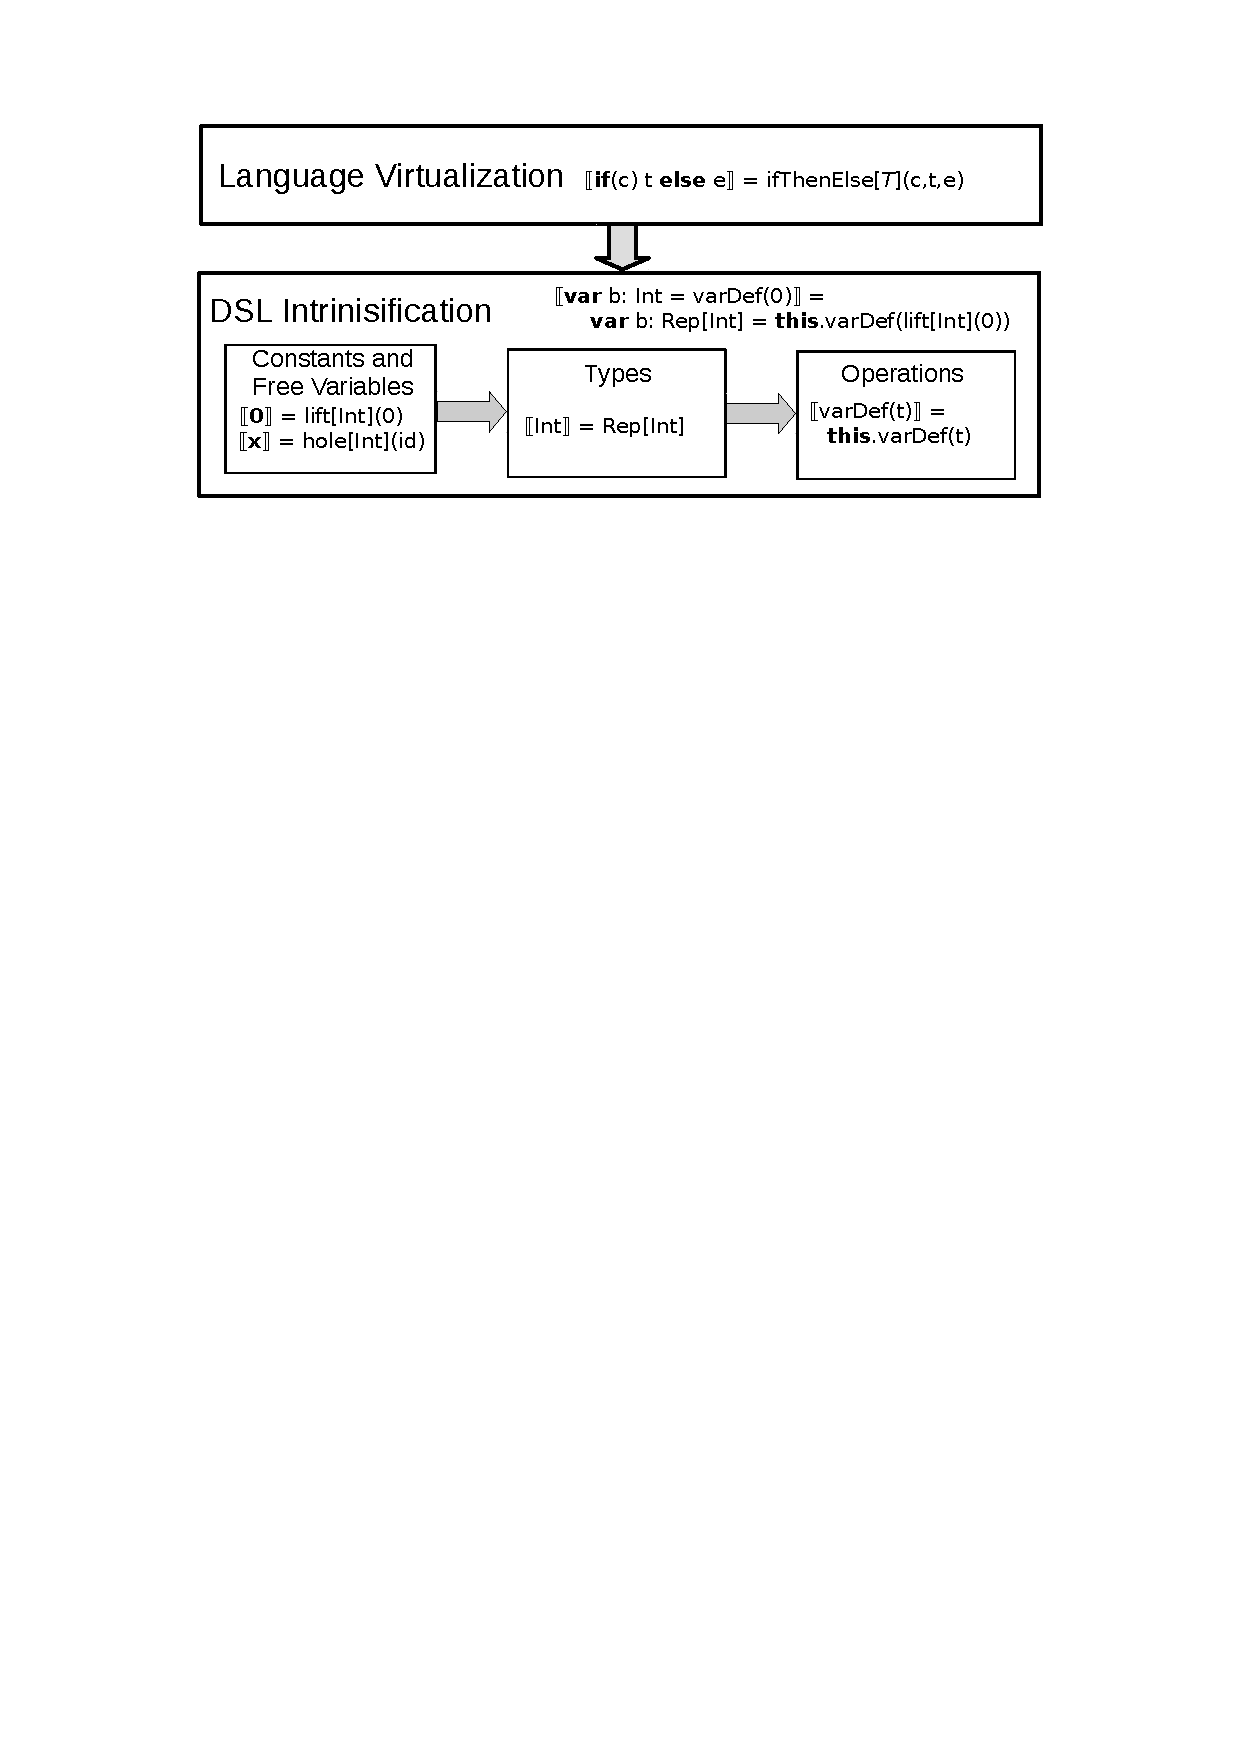
\includegraphics{diagrams/pipeline.pdf}
\caption{Translation from the direct to the deep embedding.}
\label{fig:pipeline}
\end{figure*}


\section{Language Virtualization}
\label{sec:langauge-virtualization}
Language virtualization allows to redefine intrinsic constructs of the
host language, such as \code{if} and \code{while} statements. This can be
achieved by translating them into suitable method invocations as shown by of Carette et al.~\cite{carette_finally_2009} and Rompf et al. in the modified Scala compiler named Scala-Virtualized~\cite{rompf_scala-virtualized:_2009}.

 \yy follows the ideas of Scala-Virtualized but virtualizes all Scala language constructs that
  appear as expressions; uses macros of unmodified Scala to virtualize its intrinsics.
  Practice has shown that DSL authors are reluctant to use a modified compiler and that for the wide adoption
  of embedded DSLs it is important to provide a solution based on unmodified Scala.

 Compared to Scala-Virtualized we translate additional language constructs:
  function/method definition and function application, exception handling, and all kinds of value-binding constructs
  (i.e., values, lazy values, and variables). Translation rules for supported language constructs are
  represented in~\figref{fig:virt-core} with $\ttrone{t}$ denoting the translation of a term $t$. In some expressions
  the original types are introspected and used as a type argument of the corresponding virtualized method. These
  generic types are later translated to the deep embedding during the DSL intrinsification phase.

  \begin{figure}[!ht]
%
%  Functions
%
    \judgement{Function Virtualization}{}

\begin{multicols}{2}
    \infyy{}
      {\tctx{\Gamma}{t: T_2}}
      {x: T_1 \Rightarrow t}{\mathtt{lam}[T_1,T_2](x: T_1 \Rightarrow \trone{t})}

    \infyy{}
      {\tctx{\Gamma}{t_1:\;\Func{T_1}{T_2} \quad t_2: \; T_1}}
      {t_1(t_2)}{\mathtt{app}[T_1,\;T_2](\ttrone{t_1},\; \ttrone{t_2})}
\end{multicols}

\vspace{1.5em}
\judgement{Method Virtualization}{}
\vspace{1em}

   \infyyax{}
      {\mathbf{def}\;f[T_1](x:T_2):T_3 {=} t}{\mathbf{def}\;f[T_1]:(T_2 {\Rightarrow} T_3){=}\trone{x:T_2 {\Rightarrow} t}}

    \infyy{}
      {\tctx{\Gamma}{t_1.f: [T_1](\Func{T_2}{T_3})}}
      {t_1.f[T_1](t_2)}{\mathtt{app}[T_2,T_3](\ttrone{t_1}.f[T_1],\ttrone{t_2})}
%
% Control constructs
%
\vspace{1.5em}
\judgement{Control Constructs}{}
\vspace{1em}
    \infyy{}
      {\tctx{\Gamma}{\mathbf{if}(t_1) \;t_2\; \mathbf{else}\;t_3: T}}
      {\mathbf{if}(t_1) \;t_2\; \mathbf{else}\;t_3}{\mathtt{ifThenElse}[T](\ttrone{t_1}, \ttrone{t_2}, \ttrone{t_3})}

    \infyy{}
          {\tctx{\Gamma}{\mathbf{try}\;t_1\;\mathbf{catch}\;t_2\;\mathbf{finally}\;t_3:\;T }}
          {\mathbf{try}\;t_1\;\mathbf{catch}\;t_2\;\mathbf{finally}\;t_3\; }{\mathtt{try}[T](\ttrone{t_1},\;\ttrone{t_2},\;\ttrone{t_3})}
    \vspace{0.05em}

\begin{multicols}{2}
    \infyyax{}
      {\mathbf{while}(c)\;b}{\mathtt{whileDo}(\ttrone{c},\;\ttrone{b})}

    \infyyax{}
      {\mathbf{do}\; b \;\mathbf{while}(c)}{\mathtt{doWhile}(\ttrone{c},\;\ttrone{b})}
\end{multicols}

    \infyyax{}
      {\mathbf{return}\; t}{\mathtt{ret}(\ttrone{t})}

%
% Varibles
%
\vspace{1.5em}
\judgement{Value Bindings}{}
\vspace{1em}

\infyyax{}
      {\mathbf{lazy\;val}\;x:T = t}{\mathbf{val}\;x:T = \mathtt{lazyValDef}[T](\ttrone{t})}

\begin{multicols}{2}
    \infyyax{}
      {\mathbf{val}\;x:T = t}{\mathbf{val}\;x:T = \mathtt{valDef}[T](t)}

    \infyyax{}
      {\mathbf{var}\;x:T = t}{\mathbf{val}\;x:T = \mathtt{varDef}[T](\ttrone{t})}
\end{multicols}

\begin{multicols}{2}
    \infyy{}
      {\tctx{\Gamma}{x: T}}
      {x}{\mathtt{read}[T](\ttrone{x})}

    \infyy{}
      {\tctx{\Gamma}{x: T}}
      {x = t}{\mathtt{assign}[T](x, \ttrone{t})}
\end{multicols}

\caption{Rules for virtualization of Scala language intrinsics.}
\label{fig:virt-core}
\end{figure}


% Binding taken care of by DSL intrinsification.
 Defined translation rules convert language constructs into method calls where each language construct has
  a corresponding method. The signature of each method is partially defined by \yy. Method names, the number of
  type parameters and the number of type arguments are predefined while types of arguments and return types
  are open for the DSL author to define (\S \ref{sec:deep-embedding-implementations}).

 Binding of the translated language constructs to the corresponding methods
  in the deep embedding is achieved during DSL intrinsification; language virtualization is
  agnostic of this binding. Further, in the implementation, all method names are prepended with $\$$
  \footnote{In Scala it is a convention that user defined method's names should not contain $\$$ characters as those are reserved for the name mangling performed by the Scala compiler.} which avoids collisions with other user functions.

 % Discuss the function translation.
 \paragraph{Functions.} We virtualize function definition and application to support full abstraction over the host
  language expressions. This allows DSL authors to define how functions are treated by
  reifying them and optionally providing analysis and transformations over them. For example, DSL authors
  can define different inlining strategies, perform call graph analysis, or instrument all function calls. With Scala-Virtualized this is not possible as functions are not translated and thus it is impossible to
  abstract over them.

% Discuss method translations.
 \paragraph{Methods.} Method definitions follow a similar philosophy as functions.
  The difference is that in Scala, the \code{def} keyword is used to define universal quantification and possibly recursion.
  This is similar to the \code{let} and \code{letrec} constructs in other functional languages. This translation is optional
  as in some DSLs it is more concise to reuse method application of the host language.

  %\toimplement

% Discuss control structures.
 \paragraph{Control constructs.} We translate all Scala control constructs (e.g.,\code{if} and \code{try} to method calls.
  Scala's type system supports parametric polymorphism, by-name parameters, and partial functions that can model
  the semantics of all control constructs. How these features are used to model the original constructs is presented in \S \ref{sec:deep-embedding-implementations}).

% Discuss variables.
 \paragraph{Value bindings.} Scala has multiple constructs for value binding: values, variables, and lazy values. \yy translates
  definition of all values into methods as well as accesses to them. Abstraction over values accesses is
  necessary for tracking effects in case of variables, access order in case of lazy values, and for instrumentation
  in case of simple values.

 \paragraph{Universal methods.} Scala is designed such that the types \code{Any} and
 \code{AnyRef}, which reside at the top of the Scala class hierarchy, contain
 \code{final} methods. Through inheritance, these methods are defined on all
 types making it impossible to override their functionality without translation.

 \yy virtualizes all methods on types \code{Any} and \code{AnyRef}. Method calls on objects
  are translated into the representation where the \code{this} pointer is passed as the first argument and, by convention, all methods start
  with a prefix \code{infix_}.

  This representation is convenient for methods that are defined once for the whole hierarchy as
  the DSL author needs to define this method only once, as opposed to adding it to each data type. The caveat with
  this approach is that in case of methods that are overridden the virtual dispatch must be
  performed manually by the DSL author.

  For DSLs that require extension of these methods we provide an alternative translation
  of universal methods into the name mangled infix form:%\toimplement

  \infyyax{}
      {t_1\; == \;t_2}{\trone{t_1}.\;\mathtt{\$==}(\;\trone{t_2})}

  \paragraph{The \code{new} construct.} The new construct of Scala can not be
  virtualized to a single method as signatures of data-type constructors differ in number
   of type arguments, the number of arguments and in their types. If the method name was the
   same for all data types the method would have to have a different type signature based on
   one of its type arguments. In Scala this would be possible with by using a combination of
   overloading and implicit parameters but this requires usage of complicated constructs in the deep embedding.


   % We wirtualize new
   Instead, we rely on the power of the translation, and we virtualize constructor calls
     to method calls whose name depends on the type that is being constructed:

  \infyy{}
      {\tctx{\Gamma} methodName = \mathtt{"new\_"} + \mathtt{path}(type)}
      {\mathbf{new} \; type[T](arg)}{methodName[T](\trone{arg})}

\begin{figure}[!ht]
%
% Virtualization of `Any` methods
%
% *   t == t1                =>       infix_==(t, t1)
\judgement{Methods on the \code{Any} type}{}
\begin{multicols}{2}
    \infyyax{}
      {t_1\; == \;t_2}{\mathtt{infix\_==}(\trone{t_1},\;\trone{t_2})}

% *   t != t1                =>       infix_!=(t, t1)
    \infyyax{}
      {t_1\;!=\;t_2}{\mathtt{infix\_!=}(\trone{t_1},\;\trone{t_2})}
\end{multicols}

% *   t.##                   =>       infix_##(t)
\begin{multicols}{2}
    \infyyax{}
      {t.\#\#}{\mathtt{infix\_\#\#}(\trone{t})}
    \infyyax{}
      {t.\mathtt{getClass}}{\mathtt{infix\_getClass}(\trone{t})}
\end{multicols}

% *   t.isInstanceOf[T]      =>       infix_isInstanceOf[T](t)
    \infyyax{}
      {t.\mathtt{isInstanceOf[T]}}{\mathtt{infix\_isInstanceOf[T]}(\trone{t})}

% *   t.asInstanceOf[T]      =>       infix_asInstanceOf[T](t)
    \infyyax{}
      {t.\mathtt{asInstanceOf[T]}}{\mathtt{infix\_asInstanceOf[T]}(\trone{t})}

%
% Virtualization of `AnyRef` methods
%
\vspace{1em}
\judgement{Methods on the \code{AnyRef} type}{}

 \begin{multicols}{2}
 % *   t eq t1                =>       infix_eq(t, t1)
   \infyyax{}
     {t_1\;\mathtt{eq}\;t_2}{\mathtt{infix\_eq}(\trone{t_1},\;\trone{t_2})}

 % *   t ne t1                =>       infix_ne(t, t1)
   \infyyax{}
     {t_1\;\mathtt{ne}\;t_2}{\mathtt{infix\_ne}(\trone{t_1},\;\trone{t_2})}
\end{multicols}

\begin{multicols}{2}

% *   t.notify               =>       infix_notify(t)
   \infyyax{}
     {t.\mathtt{notify}}{\mathtt{infix\_notify}(\trone{t})}

% *   t.notifyAll            =>       infix_notifyAll(t)
   \infyyax{}
     {t.\mathtt{notifyAll}}{\mathtt{infix\_notifyAll}(\trone{t})}
\end{multicols}

\begin{multicols}{2}
% *   t.wait                 =>       infix_wait(t)
   \infyyax{}
     {t.\mathtt{wait}}{\mathtt{infix\_wait}(\trone{t})}

    % *   t.wait(l)              =>       infix_wait(t, l)
  \infyyax{}
     {t_1.\mathtt{wait}(t_2)}{\mathtt{infix\_wait}(\trone{t_1},\;\trone{t_2})}
\end{multicols}

% *   t.wait(t1, l)          =>       infix_wait(t, t1, l)
   \infyyax{}
      {t_1.\mathtt{wait}(t_2,\;t_3)}
      {\mathtt{infix\_wait}(\trone{t_1},\;\trone{t_2},\;\trone{t_3})}

% *   t.synchronized[T](t1)  =>       infix_synchronized(t, t1)
  \infyyax{}
     {t_1.\mathtt{synchronized}[T](t_2)}
     {\mathtt{infix\_synchronized}[T](\trone{t_1},\;\trone{t_2})}

\caption{Rules for virtualization of methods on \code{Any} and \code{AnyRef}.}
\label{fig:virt-any}
\end{figure}


 \paragraph{Not virtualizing class definitions.} \yy does not virtualize class and trait definitions, including the \emph{case class}
  definitions. For the given set of DSL compiler frameworks that use \yy it was hard to identify
  an abstraction that would allow virtualization of Scala classes.

  This limitation, however, does not preclude class virtualization for embedded DSLs. We allow extensions to \yy that virtualize classes and traits through the use of the reflection API. The drawback of this approach is that DSL authors are required
  to know the reflection API compared to the simple interface of language virtualization. For now, each framework that uses \yy defines
  its own translation scheme.

 \paragraph{Configuring method virtualization.} When we virtualize methods and their application
   we effectively override all expressions of Scala. In this case the DSL author has to:
   \emph{i)} write the DSL definition in a way that corresponds to the translation and is not idiomatic to Scala,
   and \emph{ii)} do additional transformation that removes all combinations of applications over domain-specific operations.

   This can be cumbersome and we leave method virtualization as a configuration option that is
    disabled by default. This way DSL authors can write DSLs in the
    Scala idiomatic way and the \code{app}/\code{lam} pairs for DSL operations never appear in the
    DSL intermediate representation.


% Name of type translation.
\newcommand{\ttname}{\tau}

% Type translations (Vojin-style).
%\newcommand{\ttarg}[1][-]{\ttname(#1, \mathtt{arg})}     % type arguments
%\newcommand{\ttother}[1][-]{\ttname(#1, \mathtt{other})} % other

% Type translations (Sandro-style).
\newcommand{\ttarg}[1][]{\ttname_{\mathtt{arg}} \ifempty{#1}{}{(#1)}}
%\newcommand{\ttother}[1][]{\ttname_{\mathtt{oth}} \ifempty{#1}{}{(#1)}}
\newcommand{\ttother}[1][]{\ttname \ifempty{#1}{}{(#1)}}

\subsection{Virtualizing Pattern Matching}
\label{sec:virtpatmat}

% Define how it works.
The Scala compiler has a virtual pattern matcher that allows for overloading the semantics
 of the pattern matching construct. \yy reuses the functionality of this pattern matcher
 in combination with DSL intrinsification to allow reasoning about it in DSL compilers.
 In this section, for purposes of explaining DSL intrinsification, we explain the functioning
 of the virtualized pattern matcher.

% Semantics of Scala pattern matching: alternatives are interpreted with a plus and failures with a zero, and guards as filters. We also need a constructor one. Example of Option.
Scala's pattern matching can be interpreted with deconstructors and operations on the \code{Option}
 type of Scala. The successful match is represented with the \code{Some} type which is
 the monadic return of the \code{Option} monad and failures with the \code{None} type
 which is a monadic \emph{zero} operation. The pattern nesting is represented with
 the monadic \emph{bind} operation \code{flatMap}; alternation is represented with the
 \code{orElse} combinator on the \code{Option} monad which represents monadic addition. The semantics
 of Scala pattern matching can be represented completely with the operations of the zero-plus monad.

% Based on the fact that Scala pattern matching can be interpreted as a zero+ monad.
The virtual pattern matcher converts Scala pattern matching to the operations on a user-defined zero-plus monad.
A pattern match is virtualized if the object \code{__match} is defined in the scope. For the original
semantics of Scala pattern matching is defined by the object \code{__match} defined in \figref{fig:match-default}. To
virtualize pattern matching users can provide their own definitions of methods in \code{__match},
implementations of the zero-plus monad, and implementations of the case class deconstructors.

% Basic Scala
\begin{figure}[ht]
\begin{listingtiny}
object __match {
  def zero: Option[Nothing] = None
  def one[T](x: T): Option[T] = Some(x)
  def guard[T](cond: Boolean, then: => T): Option[T] =
    if(cond) one(then) else zero
  def runOrElse[T, U](x: T)(f: T => Option[U]): U =
    f(x) getOrElse (throw new MatchError(x))
}
\end{listingtiny}
\caption{The implementation of the virtualized pattern matcher with the original
 Scala semantics and with \code{Option} as the zero-plus monad.}
\label{fig:match-default}
\end{figure}


% Example of a single pattern.
If the object \code{__match} is in scope a simple pattern match\begin{lstparagraph}
p match {
  case Pair(l, r) => f(l,r)
}
\end{lstparagraph}

is translated into\begin{lstparagraph}
__match.runOrElse(p) { x1: Any =>
  Pair.unapply(x1).flatMap(x2: (Int, Int) => {
    val l: Int = x2._1; val r: Int = x2._2;
    __match.one(f(l, r))
  })
}
\end{lstparagraph}

% Example of alternation.
In case of multiple case clauses\begin{lstparagraph}
p match {
  case Pair(l, r) => f(l,r)
  case Tuple2(l, r) => f(l,r)
}
\end{lstparagraph}
the monadic addition \code{orElse} is used for matching alternative statements in order:\begin{lstparagraph}
Pair.unapply(p).flatMap(x2: (Int, Int) => {
  val l: Int = x2._1; val r: Int = x2._2;
  __match.one(f(l, r))
}).orElse(
  Tuple2.unapply(p).flatMap(x3: (Int, Int) => {
    val l: Int = x3._1; val r: Int = x3._2;
    __match.one(f(l, r))
}))
\end{lstparagraph}

% Example of guards.
Nested pattern matches\begin{lstparagraph}
p match {
  case Pair(Pair(ll, lr), r) => f(f(ll,lr), r)
}
\end{lstparagraph}

are translated into nested calls to \code{flatMap}:\begin{lstparagraph}
Pair.unapply(p).flatMap(x2: (Int, Int) => {
  val r: Int = x2._2;
  Pair.unapply(x2._1).flatMap(x4: (Int, Int) => {
    val ll: Int = x4._1; val lr: Int = x4._2;
    __match.one(f(f(ll, lr), r))
  })
})
\end{lstparagraph}

Finally the pattern guards are translated into the call to the \code{guard} function that executes the
by-name body of the case when the \code{cond} statement is satisfied.


\section{DSL Intrinsification}
\label{sec:dsl-intrinsification}

DSL intrinsification maps directly embedded versions
 of the DSL intrinsics to their deep counterparts. The constructs that
 we translate~(\figref{fig:pipeline}) are: \emph{i)} constants and
 free variables~(\S \ref{sec:constants-and-free-variables}), \emph{ii)} DSL types~(\S \ref{sec:type-translation}), and \emph{iii)} DSL operations in the direct program~(\S \ref{sec:operation-translation}).

\subsection{Constants and Free Variables}
\label{sec:constants-and-free-variables}

 \paragraph{Constants.} Constant values can be intrinsified in the deep embedding in multiple ways.
 They can be converted to a method call for each constant (e.g., $\trone{\mathtt{1}} = \mathtt{\_1}$),
  type (e.g., $\trone{\mathtt{1}} = \,$\code{liftInt(1)}), or with a unified polymorphic function (e.g., $\trone{\mathtt{1}} = \,$\code{lift[Int](1)}) that uses type classes to define behavior and the return type of \code{lift}.

  % Why do we use type classes.
  In \yy we use the polymorphic function approach for to translate constants

      \infyy{}
          {\tctx{\Gamma}{c:\;T}}
          {c}{\mathtt{lift}[T](c)}

  where $c$ is a constant. We choose this approach as DSL frameworks
  commonly have a single IR node for all constants and it is easiest to implement
  such behavior with a single lift method.

  The deep embedding can, given that Scala supports type-classes, provide an implementation
  of lift that depends on the type of $c$. The DSL author achieves this
  by providing a type class instance for lifting a set of types (defined by upper and lower bounds)
  of constants.

  % What are constants in Scala
  In \yy we treat as constants:
  \begin{enumerate}

   \item \emph{Scala literals} of all primitive types \code{Char}, \code{Short},
     \code{Int}, \code{Long}, \code{Float}, and \code{Double}, as well as literals of
      type \code{String} (\code{\"...\"}), \code{Unit} (\code{()}), and \code{Null} (\code{null}).

   \item \emph{Scala object accesses} e.g., \code{Vector} in \code{Vector.fill} is viewed as a constant. This allows
    the DSL authors to re-define the default behavior of object access. Translating objects is optional as
    leaving their original semantics simplifies the implementation of the deep embedding,
    but requires special cases in type translation.\todo{link to the examples}
  \end{enumerate}


\paragraph{Free variables.} Free variables are external variables captured by
  a direct \edsl{} term.  All that deep embedding knows about these terms is
  their type and that they will become available only during evaluation (i.e., interpretation or
  execution after code generation).  Hence, free variables need to be treated
  specially by the translation and the deep embedding needs to provide support
  for their evaluation.

  \yy tracks free variables in the DSL scope and translates them into a call to the polymorphic function \code{hole[T]}. As the arguments
  \yy passes the unique identifier for that variable:

    \infyy{}
          {\tctx{\Gamma}{x:\;T} \quad x\;\mathtt{is}\;\mathtt{a}\;\mathtt{free}\;\mathtt{variable}}
          {x}{\mathtt{hole}[T](\mathtt{uid}(x))}

  In \figref{fig:translation-example}, the free variables
  \code{n} and \code{exp} are replaced with calls to the polymorphic method
  \code{hole[T]}, which handles the evaluation of free variables in the deep
  embedding. Each captured identifier is assigned with a unique number that
  is passed as an argument to the \code{hole} method
   (0 and 1 in \figref{fig:translation-example}).
  The identifiers are later sorted and passed as arguments to the Scala function that is a result
  of \edsl compilation. The DSL author is required to ensure that the position and the type
  of the resulting function matches the order and types of the sorted identifiers passed by \yy.

\subsection{Type Translation}
\label{sec:type-translation}
 The \emph{type translation} maps every DSL type in the, already
  virtualized, term body to an equivalent type in the deep embedding.
  In other words, the type translation is a function on
  types.  Note that this function is inherently DSL-specific, and
  hence needs to be configurable by the DSL author.

  % The type mapping depends on the input type and the context. For all practical type mappings we only had to distinguish between the type-argument position (\code{arg}), e.g. \code{Int} in \code{lam[Int, Int]}, and the others (\code{other}). We define this function as $\tau: \mathbb{T} \times \mathbb{C} \rightarrow \mathbb{T}$ where $\mathbb{T}$ is the set of all types and $\mathbb{C} = \{\mathtt{arg}, \mathtt{other}\}$ denotes whether the type appears in the type-argument position. In \figref{fig:translation-example} this function transforms all types \code{T} that are not in the type-argument position to \code{Rep[T]}.

  The type mapping depends on the input type and the context. In
  practice, we need only distinguish between types in type-argument
  position, e.g. the type argument \code{Int} in the polymorphic
  function call \code{lam[Int, Int]}, and the others.  To this end, we
  define a pair of mutually recursive functions $\ttarg, \ttother
  \colon \mathbb{T} \rightarrow \mathbb{T}$ where $\mathbb{T}$ is the
  set of all types and $\ttarg$ and $\ttother$ translate types in
  argument and non-argument positions, respectively.

% Gives us a number of interesting possibilities.
  Having type translation as a function opens a number of possible deep embedding
   strategies. Alternative type translations can also dictate the interface of \code{lam}
   and \code{app} and other core \edsl{} constructs. Here we discuss the ones that we find
   useful in \edsl{} design:

\paragraph{The identity translation.}  If we choose $\ttother$ to be
the identity function and virtualization methods such as \code{lam},
\code{app} and \code{ifThenElse} to be implemented in the obvious way
using the corresponding Scala intrinsics, the resulting translation
will simply yield the original, directly embedded DSL program. Usages
of this translation are shown in \S \ref{sec:identity-embedding}.

\paragraph{Generic polymorphic embedding.} If instead we choose
$\ttother$ to map any type term $T$ (in non-argument position)
to \code{Rep[$T$]}, for some abstract, higher-kinded IR type
\code{Rep} in the deep EDSL scope, we obtain a translation to a
\emph{finally-tagless, polymorphic}
embedding~\cite{carette_finally_2009,hofer_polymorphic_2008}. For this
embedding, the translation functions are defined as:
\begin{alignat*}{2}
&\ttarg[T]   & \; = \; & T \\
&\ttother[T] & \; = \; & \text{\code{Rep[}} T \text{\code{]}}
\end{alignat*}

By choosing the virtualized methods to operate on the IR-types in the
appropriate way, one obtains an embedding that \emph{preserves
  well-typedness}, irrespective of the particular DSL it implements.
We will not present the details of this translation here, but refer
the interested reader to~\cite{carette_finally_2009} and the description of the
 corresponding deep embedding for this translation~(\S \ref{sec:polymorphic-embedding}).

\paragraph{Eager inlining.} In high-performance EDSLs it is often desired to
eagerly inline all functions and to completely prevent dynamic dispatch in
user code (e.g., storing functions into lists).  This is achieved by translating
function types of the form \code{$A$ => $B$} in the direct embedding into
\code{Rep[$A$] => Rep[$B$]} in the deep embedding (where \code{Rep} again
designates IR types). Instead of constructing an IR node for function application, such functions reify the
whole body of the function starting with IR nodes passed as arguments. The effect of such
reification is equivalent to inlining. This function representation is used in LMS~\cite{rompf_lightweight_2012} by default
and we use it in \figref{fig:translation-example}. The translation functions are defined as:
\renewcommand*{\mathellipsis}{%
  \mathinner{{\ldotp}{\ldotp}{\ldotp}}%
}
\begin{alignat*}{3}
&\ttarg[T\lbrack I_1,\ldots,I_n \rbrack]   & \; = \; & T[\ttarg[I_1],\ldots,\ttarg[I_n]] \\
&\ttarg[T_1 \Rightarrow T_2] & \; = \; & \mathtt{error} \\
&\ttarg[T] & \; = \; & T, \; \text{otherwise} \\ % \text{if } T \notin \{T_1 \Rightarrow T_2, T[I_1,\ldots,I_n]\} \\
%&\ttother[T_1 \Rightarrow T_2] & \; = \; & \ttother[T_1] \Rightarrow \ttother[T_2]\\
&\ttother[T_1 \Rightarrow T_2] & \; = \; & \text{\code{Rep[}}\ttarg[T_1]\text{\code{]}} \Rightarrow \text{\code{Rep[}}\ttarg[T_2]\text{\code{]}}\\
&\ttother[T] & \; = \; & \text{\code{Rep[}} T \text{\code{]}},
\; \text{otherwise}
\end{alignat*} %\text{if } T \neq T_1 \Rightarrow T_2

This translation preserves well-typedness but rejects programs that contain
function types in the type-argument position. In this case this is a desired
behavior as it fosters high-performance code by avoiding dynamic dispatch. As an alternative to rejecting function types in the type-argument position the deep embedding can provide
coercions from \code{Rep[$A$] => Rep[$B$]} to \code{Rep[$A$ => $B$]} and from \code{Rep[$A$ => $B$]} to \code{Rep[$A$] => Rep[$B$]}.

This translation disallows usage of curried functions in the direct programs. If we
represent the curried functions as the polymorphic types then
functions would appear in the type argument position. To re-introduce the curried functions we
provide a translation with the modified rule for translation of functions:
\begin{alignat*}{3}
&\ttother[T_1 \Rightarrow T_2] & \; = \; & \ttother[T_1] \Rightarrow \ttother[T_2]\\
\end{alignat*} %\text{if } T \neq T_1 \Rightarrow T_2
which is correct only when the virtualization of functions and methods is disabled.

\paragraph{Custom types.} All previous translations preserved types in the type parameter position. The reason is that the $\ttname$ functions behaved like a higher-kinded type. If we would like to map some of the base types in a custom way, those types need to be changed in the position of type-arguments as well. This translation is used for \edsls based on polymorphic embedding~\cite{hofer_polymorphic_2008} that use \code{this.T} to represent type \code{T}.

This translation simply prepends each type with a prefix (e.g., \code{this}) so that
the deep embedding can redefine it:
\begin{alignat*}{3}
&\ttarg[T] & \; = \; & this.T\\
&\ttother[T] & \; = \; & this.T\\
\end{alignat*}

Unlike with the previous translations, where the type system of the direct embedding was
ensuring that the term will type-check in the deep embedding, this translation gives no guarantees. The
responsibility for the correctness of the translation is on the DSL author. The deep embedding
for this translation is presented in \S \ref{sec:embedding-with-custom-types} and we applied
this translation for embedding Slick \cite{slick} with great success~(\S \ref{subsec:slick}).

\paragraph{Untyped backend.} If DSL authors want to avoid complicated types in the back-end (e.g., \code{Rep[T]}), the $\ttname$ functions can simply transform all types to the \code{Dynamic}~\cite{abadi_dynamic_1991} type. Giving away type safety can make transformations in the back-end easier for the DSL author.

\paragraph{Changing the translation.} By simply changing the type translation, the \edsl author can modify behavior of an \edsl.  For example, with the generic polymorphic embedding the \edsl will reify function IR nodes and thus allow for dynamic dispatch. In the same \edsl that uses the eager inlining translation, dynamic dispatch is restricted and all function calls are inlined.

\subsection{Operation Translation}
\label{sec:operation-translation}

The \emph{operation translation} maps directly embedded versions of the
  DSL operations into corresponding deep embeddings. To this end, we define a
  function \code{opMap} on terms that returns a deep operation for each directly
  embedded operation.

The \code{opMap} function in Scala intrinsifies direct \edsl body in the context of the deep embedding.
 \code{opMap} can be defined as a composition of two functions: \emph{i)} function \code{inject} that inserts the direct \edsl body
  into a context where deep \edsl definitions are visible, and \emph{ii)} \code{rebind}
  rebinds operations of the direct \edsl to the operations of the deep \edsl. Function \code{opMap} is equivalent to
  the composition of \code{inject} and \code{rebind} (written in Scala as \code{rebind andThen inject}).

\paragraph{Operation \code{rebind}.} Operations in Scala are resolved through a \emph{path}. For example, a call to the \code{println} method
  of the Scala object \code{Predef}\begin{lstparagraph}
scala.collection.immutable.Vector.fill(1)(42)
\end{lstparagraph}
  has a path \code{scala.collection.immutable.List.fill}\footnote{Scala packages have a hidden prefix \code{_root_} that we always omit for simplicity.}.

This phase of the translation translates paths of all operations so they bind
 to operations in the deep embedding. The translation function can perform an
 identity operation, prefix addition, name mangling of function names, etc.


\paragraph{Operation \code{inject}.} For \yy and polymorphic embeddings~\cite{hofer_polymorphic_2008}
in general we chose to inject the body of our DSLs into the refinement of the Scala component that
contains all deep DSL definitions

  \infyyax{}
   {dsl}{\mathbf{new}\;\;de\;\;\{\;\;\mathbf{def}\;\;\mathtt{main}():\;\;\ttother[T]\;=\;dsl\;\}}

where $dsl$ is the direct DSL program after rebinding and $de$ is the component name
that is provided by the DSL author that holds all definitions in the deep embedding, and
$\tau$ is the type translation.

Alternatively the DSLs can be injected into the scope by importing all DSL operations
 from the object that contains the deep embedding definitions.

  \infyyax{}
    {dsl}{\mathbf{val}\;\;c \; = \; \mathbf{new}\;\;de;\;\;\;\mathbf{import}\;\;c.\_;\;\;\;dsl}

In both cases the corresponding \code{rebind} function can be left as an
identity. If the deep embedding has all the required methods with corresponding
 signatures all operations will rebind to the
operations of the deep embedding by simply re-type-checking the program in the new context.

% Example
For example in a simple function application\begin{lstparagraph}
Vector.fill(1)(42)
\end{lstparagraph}the injection will rebind the operation through the extension methods of Scala. The
resulting code will contain wrapper classes that extend DSL types with deep operations:\begin{lstparagraph}
VectorOps(lift(Vector)).fill(lift(1))(lift(42))
\end{lstparagraph}

% Talk about additional implicit parameters.
Finally injection in the DSL scope allows the deep embedding to introduce additional implicit arguments to
 all DSL operations. The implicit arguments introduced in the direct embedding are treated
 as explicit in the deep embedding. For example, the \code{fill} operation can be augmented
 with the source information from the direct embedding and run-time type representation:\begin{lstparagraph}
VectorOps(lift(Vector)).fill(lift(1))(lift(42))(
  sourceContext("example.scala",1,1), typeTag[Int]
)
\end{lstparagraph}

% Important the DSL author can use a convenient interface for DSL designing DSL internals.
In \yy we chose the operation translations that closely match the structure of
 the direct embeddings. This allows the authors of the deep embedding to use the
 DSL itself for development of new DSL components. In this case the DSL author can use
 the deep interface augmented with implicit conversions that all simplify lifting constants,
 calling operations etc. With such interface the previous example resembles the direct embedding\begin{lstparagraph}
Vector.fill(1)(42)
\end{lstparagraph}
except for the abstraction leaks of the deep embedding (\S \ref{sec:abstraction-leaks}).
This approach requires less code than than ``naked'' AST manipulation\todo{cite}, e.g:\begin{lstparagraph}
VectorFill(Const(1), Const(42))
\end{lstparagraph}

\todo{calling the methods}

\subsection{Translation as a Whole}
\label{sec:translation-example}

To present the translation as a whole we use an example program for calculating $\sum_{i=0}^n i^{exp}$ using the vector \edsl defined in \figref{lst:vector}. \figref{fig:translation-example} contains three versions of the program: \figref{lst:direct-embedding} depicts the direct embedding version, \figref{lst:desugaring} represents the program after type checking\footnote{The Scala type-checker modifies the program by resolving identifiers to their full paths, adding implicit parameters, etc.} (as the translation sees it), and \figref{lst:transformed_program} shows the result of the translation.

In~\figref{lst:transformed_program} we see two divergences we omitted from the translation rules for clarity:\begin{itemize}

\item All translated methods are prepended with \code{$\$$}. They are added to the code as this makes translation specific methods treated specially by the Scala tool-chain. Methods with $\$$ are invisible in the deep embedding documentation, REPL, and IDE code auto-completion.

\item The method \code{$\$$hole} is not populated with type parameters but it has a call to \code{$\$$tpe} added as a second argument. This is added as in Scala one can not provide partial
type arguments to the method and the idea of \yy is to leave the definition of \code{$\$$hole} open to the DSL authors. With \code{$\$$tpe} added Scala's type-inference can infer the type parameters of method \code{$\$$hole}. Similarly \code{$\$$lift} is not provided by the type
parameter but the type is provided by the first argument.

\end{itemize}


In~\figref{lst:transformed_program}, on line 2 we see the DSL component in which
 the DSL program is injected. On line 3 we see how Scala's \code{if} is virtualized
 to \code{$\$$ifThenElse}. On line 4, in the condition, \code{n} as it is a captured variable
 is lifted to the call to \code{$\$$hole(0, $\$$tpe[Int])} as it is a captured variable
 and the identifier \code{0} as it shows as the first variable in the DSL program. On the same line constant \code{0} is lifted to \code{$\$$ lift(0)}. On line 5 we see how the type
 of the \code{val} is translated transformed to \code{Rep[Vector[Int]]} and how
 \code{val} is virtualized. On line 6 \code{vector.Vector} is lifted as a constant.
 On line 7 we see how variable \code{n} is replaced with a hole with the same identifier (\code{0}). This identifier communicates to the deep embedding that it is the same value.
 On line 8 the Scala function is virtualized to the \code{$\$$lam} call. On line
 9 the identifier \code{exp} is translated to \code{$\$$hole(1, $\$$tpe[Int])} (with the identifier \code{1}) as
 \code{n} appears as the second identifier in the program.


\begin{figure*}[!ht]
\begin{multicols}{2}
\begin{subfigure}[b]{1\linewidth}
\centering
\vspace{1.80em}
\begin{listingtiny}
import vector._
import math.pow
val n = 100; val exp = 6;
vectorDSL {
  if (n > 0) {
    val v = Vector.range(0, n)
    v.map(x => pow(x, exp)).sum
  } else 0
}
\end{listingtiny}
\vspace{1.80em}
\caption{A program in direct embedding for calculating $\sum_{i=0}^n i^{exp}$.}
\label{lst:direct-embedding}
\end{subfigure}
\lstset{numbers=left,xleftmargin=2em,framexleftmargin=1.5em}
\begin{subfigure}[b]{1\linewidth}
\centering
\begin{listingtiny}
val n = 100; val exp = 6;
vectorDSL {
  if (n > 0) {
    val v: Vector[Int] =
      vector.Vector.range(0, n)
    v.map[Int](x: Int =>
      math.`package`.pow(x, exp)
    ).sum[Int](
      math.Numeric.IntIsIntegral)
  } else 0
}
\end{listingtiny}
\caption{The original program after desugaring and type inference.}
\label{lst:desugaring}
\end{subfigure}

\end{multicols}
\lstset{numbers=left,xleftmargin=2em,framexleftmargin=1.5em}
\begin{subfigure}[b]{1\linewidth}
\begin{listingtiny}
val n = 100; val exp = 6;
new VectorDSL with IfOps with MathOps { def main() = {
  $\$$ifThenElse[Int](
    $\$$hole(0, $\$$tpe[Int]) > $\$$lift(0),{ // then
    val v: Rep[Vector[Int]] = $\$$valDef[Vector[Int]](
      $\$$lift(vector.Vector).range(
        $\$$lift(0), $\$$hole($\$$tpe[Int], 0)))
    v.map[Int]($\$$lam[Int, Int](x: Rep[Int] =>
      $\$$lift(math.`package`).pow(x, $\$$hole($\$$tpe[Int], 1))
    ).sum[Int]($\$$lift(math.Numeric).IntIsIntegral)
  },{ // else
    $\$$lift(0)
  })
}
\end{listingtiny}
\caption{The \yy translation of the program from \figref{lst:desugaring}.}
\label{lst:transformed_program}

\end{subfigure}
\caption{\label{fig:translation-example} Transformation of an EDSL program for calculating $\sum_{i=0}^n i^{exp}$.}
\end{figure*}

\subsection{Correctness}
\label{sec:correctness}
To completely conceal the deep embedding all type errors must be captured in the direct embedding or by the translation, i.e., the translation must never produce an ill-typed program. Proving this property is verbose and partially covered by previous work. Therefore, for each version of the type translation we provide references to the previous work and give a high-level intuition:
\begin{itemize}

\item \emph{The identity translation} ensures that well-typed programs remain
well typed after the translation to the deep embedding
\cite{carette_finally_2009}. Here the deep embedding is the direct embedding
with virtualized host language intrinsics.

\item \emph{Generic polymorphic embedding} preserves well-typedness~\cite{carette_finally_2009}.
 Type \code{T} is uniformly translated to \code{Rep[T]} and thus every term will conform to its expected type.

\item \emph{Eager inlining} preserves well-typedness for programs that are
not explicitly rejected by the translation. We discuss correctness of eager inlining
in the appendix on a Hindley-Milner based calculus similar to the one of Carette et al.~\cite{carette_finally_2009}.

For the intuition why type arguments can not contain function types consider passing an increment function to the generic identity function:\begin{lstparagraph}
  id[T => T](lam[T, T](x => x + 1))
\end{lstparagraph}
Here, the \code{id} function expects a \code{Rep[_]} type but the argument is \code{Rep[T] => Rep[T]}.

\item The \emph{Dynamic} type supports all operations and, thus, static type errors will not occur. Here, the DSL author is responsible for providing a back-end where dynamic type errors will not occur.

\item \emph{Custom types} can cause custom type errors since \edsl authors can
arbitrarily redefine types (e.g., \code{type Int = String}. \yy provides
\emph{no guarantees} for this type of the translation.

%\toimplement Generics

\end{itemize}

\section{Translation in the Wider Context}
\label{sec:other-languages}

% Staging and partial evaluation

\yy consistently translates terms to the embedded domain and, thus, postpones
DSL compilation to run-time. Although, compilation happens in a different
compilation stage, \yy does not allow staging~\cite{taha_multi-stage_1997}.
\edsls can, however, achieve partial evaluation~\cite{jones1993partial} if their
implementation supports it.

% Yin-Yang requires a few things.
We implemented \yy in Scala, however, the underlying principles are applicable
in the wider context. \yy operates in the domain of statically typed languages
based on the Hindley-Milner calculus with a type system that is advanced enough
to support deep DSL embedding. The type inference mechanism, purity, laziness,
and sub-typing, do not affect the operation of \yy. Different aspects of \yy
require different language features, which we discuss separately below.

% For the translation (nice interface) type introspection. For the library macros.
\paragraph{The core translation} is based on term and
type transformations. Thus, the host language must support reflection,
introspection and transformation on types and terms. This can be achieved both
at run-time and compile-time.

% Semantic Equivalence
\paragraph{Semantic equivalence} between the direct embedding and deep embedding
is required for debugging and prototyping. If there is a \emph{semantic mismatch}~\cite{czarnecki_dsl_2004}
 between the two embeddings, e.g., the host language is lazy and the embedded
 language is strict, \yy can not be used for debugging. In this scenario the
 direct embedding can be implemented as stub which is used only for its user
 friendly interface and error reporting.

%%%%%%%%%%%%%%%%%%%%%%%%%%%%%%%%%%%%%%%%%%%%%%%%%%%%%%%%%%%%%%%%%%%%%%%%%%%%%%%
%                           Deep Embedding with Yin-Yang
%%%%%%%%%%%%%%%%%%%%%%%%%%%%%%%%%%%%%%%%%%%%%%%%%%%%%%%%%%%%%%%%%%%%%%%%%%%%%%%
\chapter{Deep Embedding with \yy}
\label{sec:deep-embedding-implementations}

The translation to the deep embedding assumes existence of an adequate deep embedding. This deep embedding
should have an interface that corresponds to: \emph{i)} methods emitted by language virtualization,
\emph{ii)} translation of constants and free variables, and \emph{iii)} DSL operations defined in
 the direct embedding.

 For each type translation, interface of the deep embedding and IR reification is
  achieved differently. In this section we describe
  how to define the deep embedding interface~(\S \ref{sec:relaxed-interface}) and achieve reification
  for relevant type translations:
   \emph{i)} the identity translation~(\S \ref{sec:identity-embedding}),
   \emph{ii)} the polymorphic embedding~(\S \ref{sec:polymorphic-embedding}),
   \emph{iii)} the polymorphic embedding with eager inlining~(\S \ref{sec:polymorphic-embedding-with-eager-inlining}), and
   \emph{iv)} the embedding with custom types~(\S \ref{sec:embedding-with-custom-types}).
  Finally, we discuss how the deep embedding is compiled and executed~(\S \ref{sec:yy-interface}). For conciseness,
   in all embeddings we omit the interface of pattern matching and virtualized universal methods.

\section{Relaxed Interface of the Deep Embedding}
\label{sec:relaxed-interface}

The \yy translation requires a certain interface from the deep embedding. This interface, however,
 does not conform to the typical definition of an interface in object oriented programming languages.
 In most translation rules only the method name, number of type arguments, and number
 of explicit arguments is defined.

The number of implicit arguments and the return type are left open for
 the DSL author to define. The implicit parameters are added by the type-checker
 after the operation translation phase if they are present in the deep embedding.
 For example, if we define the \code{$\$$ifThenElse} function as\begin{lstparagraph}
def $\$$ifThenElse[T](cond: Boolean, thn: => T, els: => T)(
  implicit tpe: TypeTag[T]): T = \\...
\end{lstparagraph}
after the translation the Scala type-checker will provide the arguments that
carry run-time type information.

This feature can be used in the deep embeddings for various purposes. The ones that
were used in DSLs based on \yy and LMS are: \emph{i)} tracking type information, \emph{ii)} tracking
positions in the source code of the direct embedding, \emph{iii)} changing the method return type
based on its argument types, and \emph{iv)} allowing multiple methods with the
same erased signature (\S \ref{sec:scala-specific-problems}).


\section{Embedding for the Identity Translation}
\label{sec:identity-embedding}

The DSL embedding for the identity translation is not truly a deep embedding. The
types are unmodified and, thus, can not represent the DSL intermediate representation.
This translations is still interesting as a mechanism for instrumenting language
constructs of Scala. The basic interface that contains all the language features,
 without any additional implicit parameters, is defined in~\figref{fig:interface-identity-dsl}.

% Control flow is preserved with the Scala by-name parameters.
With this embedding the order of execution in all control flow constructs of Scala is preserved with
 by-name parameters. For example, in \code{$\$$ifThenElse} both the \code{thn} and the \code{els} parameters
are by-name and their execution order is defined by the implementation of the method. Similarly,
\code{$\$$whileDo}, \code{$\$$doWhile}, \code{$\$$try}, and \code{$\$$lazyValDef} have their
 parameters by-name.

The DSL author can instrument Scala language features by re-defining virtualized methods. For example,
 collecting profiles of \code{if} conditions can be simply added by overriding the
\code{$\$$ifThenElse} method:\begin{lstparagraph}
def $\$$ifThenElse[T](cond: Boolean, thn: => T, els: => T)(
  implicit sc: SourceContext): T = {
  val (thnCnt: Long, elsCnt: Long) =
    globalProfiles.getOrElse(sc, (0, 0))

  globalProfiles.update(sc,
    if (cond) (thnCnt + 1, elsCnt)
    else (thnCnt, elsCnt + 1))
  if (cond) thn else els
}
\end{lstparagraph}

Achieving the same effect with a facility like macros would require the DSL author to know the
reflection API of Scala which involves details about the Scala intermediate representation.
Further, the DSL author would be required to write transformers of that intermediate representation.

Supported features that are not of interest in the deep embedding
 can be removed with an interesting trick. If we implement each method in the deep embedding as a macro
 that inlines the method to its original language construct all abstraction overhead of virtualized methods
 disappears. For example, \code{$\$$ifThenElse} can be returned to a regular if with\begin{lstparagraph}
def $\$$ifThenElse[T](cond: Boolean, thn: => T, els: => T): T =
  macro ifThenElseImpl[T]

def ifThenElseImpl[T](c: Context)(cond: c.Tree,
  thn: c.Tree, els: c.Tree): c.Tree = { import c.universe._
  q"if ($\$$cond) $\$$thn else $\$$els"
}
\end{lstparagraph}

\yy provides a Scala component that has methods of all language features overridden with macros that rewrite
 them to the original language construct. By using this component the DSL author can override functionality
of individual language constructs without a need to redefine all other language features.

% Hole and lift interface.
In \figref{fig:interface-identity-dsl} method \code{hole} has a slightly different  representation than what is presented in \S \ref{sec:translation}. Method \code{hole}
 has an additional parameter for the run-time type information~(\code{tpe: TypeTag[T]}).
 This parameter is passed explicitly by \yy to allow the compiler to infer the type arguments
 of the method hole. This allows additional freedom for defining the interface of hole~(see \todo{embedding with custom types}).


\begin{figure}
\begin{listingtiny}
trait FunctionsInterface {
  // only a subset of function arities is displayed
  def $\$$app[U](f: () => U): () => U
  def $\$$lam[U](f: () => U): () => U

  def $\$$app[T_1, U](f: T_1 => U): T_1 => U
  def $\$$lam[T_1, U](f: T_1 => U): T_1 => U
}

trait IdentityInterface with FunctionsInterface {
  // constants and captured variables
  def lift[T](v: T): T
  def hole[T](id: Long, tpe: TypeTag[T]): T

  // control structures
  def $\$$ifThenElse[T](cond: Boolean, thn: => T, els: => T): T
  def $\$$return(expr: Any): Nothing
  def $\$$whileDo(cond: Boolean, body: => Unit): Unit
  def $\$$doWhile(body: => Unit, cond: Boolean): Unit
  def $\$$try[T](body: => T, catches: Throwable => T, fin: => T): T
  def $\$$throw(t: Throwable): Nothing

  // variables
  def $\$$valDef[T](init: T): T
  def $\$$lazyValDef[T](init: => T): T
  def $\$$varDef[T](init: T): T
  def $\$$read[T](init: T): T
  def $\$$assign[T](lhs: T, rhs: T): Unit
}
\end{listingtiny}
\caption{Interface of the identity DSL.}
\label{fig:interface-identity-dsl}
\end{figure}



\section{Polymorphic Embedding}
\label{sec:polymorphic-embedding}

% Explain the polymorphic embedding.
With the generic polymorphic embedding we uniformly abstract over each type in the
 direct embedding. This abstraction can be used to give different semantics
 (thus polymorphic) to the deep programs. In the context of the deep DSLs the most
 common semantics is reification of the intermediate representation.

% More on polymorphic embedding.
In \figref{fig:polymorphic-embedding} we show the basic interface
 for the generic polymorphic embedding. In trait
 \code{PolymorphicBase} the type \code{R[+T]}\footnote{Some deep
 embeddings call this type \code{Rep}, \code{Repr}. We use the name \code{R} as in
 languages with local type inference this type is omnipresent in method signatures and makes them longer.} is the abstraction over the types in the direct embedding. This type is covariant in type \code{T}
 and therefore the abstract types have the same subtyping relation as the types
 in the direct embedding.

In this embedding both function definition and function application are abstracted over.
 \code{lam} converts functions from the host language into the functions in the embedded language and
 \code{app} returns functions from the embedded language into the host language. This way the DSL author
 has complete control over the function definition/application in the deep embedding.

\begin{figure}
\begin{listingtiny}
trait PolymorphicBase { type R[+T] }

trait GenericFunctionsBase extends PolymorphicBase {
  // only a subset of function arities is displayed
  def $\$$app[U](f: R[() => U]): () => R[U]
  def $\$$lam[U](f: () => R[U]): R[() => U]

  def $\$$app[T_1, U](f: R[T_1 => U]): R[T_1] => R[U]
  def $\$$lam[T_1, U](f: R[T_1] => R[U]): R[T_1 => U]
}

trait PolymorphicInterface extends GenericFunctionsBase {
  // constants and captured variables
  def lift[T](v: T): R[T]
  def hole[T](id: Long, tpe: TypeTag[T]): R[T]

  // control structures
  def $\$$ifThenElse[T](cnd: R[Boolean], thn: => R[T], els: => R[T]): R[T]
  def $\$$return(expr: R[Any]): R[Nothing]
  def $\$$whileDo(cnd: R[Boolean], body: => R[Unit]): R[Unit]
  def $\$$doWhile(body: => R[Unit], cond: R[Boolean]): R[Unit]
  def $\$$try[T](body: => R[T], catches: R[Throwable => T], fin: => R[T]): R[T]
  def $\$$throw(e: R[Throwable]): R[Nothing]

  // variables
  def $\$$valDef[T](init: R[T]): R[T]
  def $\$$lazyValDef[T](init: => R[T]): R[T]
  def $\$$varDef[T](init: R[T]): R[T]
  def $\$$read[T](init: R[T]): R[T]
  def $\$$assign[T](lhs: R[T], rhs: R[T]): R[Unit]
}
\end{listingtiny}
\caption{Interface of the generic polymorphic embedding.}
\label{fig:polymorphic-embedding}
\end{figure}

% How one adds methods to such embedding.
Compared to the deep embeddings in Scala (e.g., LMS) the DSL author should follow the
translation rules for the deep embedding to be applicable to \yy. Similarly to deep DSLs the
DSL operation are added to \code{R[T]} types in the same manner. In addition the DSL author should:
\emph{i)} provide lifting for Scala objects and \emph{ii)} transform the bodies of deep embedding operations.

% Lifting objects
\paragraph{Objects in the deep embedding.} Objects in the deep embedding must correspond to the
translated objects in the direct embedding. Since we treat objects as constants
they are handled by the \code{lift} method.

An object from the direct embedding should be represented with an appropriate \code{lift} method and a set
 of extension methods that represent its operations. For example, to support the \code{println}
 method on the \code{Predef} object the deep embedding must introduce a lifting construct and
 an extension method on \code{R[Predef.type]}:\begin{lstparagraph}
 def lift(c: Predef.type): R[Predef.type] = Const(Predef)
 implicit class PredefOps(predef: R[Predef.type]) {
   def println(p: R[Any]): R[Unit] = \\...
 }
 \end{lstparagraph}

To preserve the original API of the deep embedding one can introduce a shortcut for the
 \code{Predef} object in the DSL component:\begin{lstparagraph}
 val Predef = lift[Predef.type](scala.Predef)
\end{lstparagraph}
This way the deep embedding can be used in a similar way to the direct embedding for
 the purpose of developing internal DSL components.


\paragraph{Operations in the direct embedding.} Implementation of the deep embedding operations
 depends on which rules of virtualiztion are applied. If we apply method virtualization
 in the DSL programs the bodes of the deep embedding operations should be transformed
 with the same transformation. For example, an identity method
 in the deep embedding\begin{lstparagraph}
   def id[T](v: R[T]): R[T] = Identity(v)
 \end{lstparagraph}
 should be transformed into\begin{lstparagraph}
   def id[T]: R[T => T] = $\$$lam[T]((x: R[T]) => Identity(v))
 \end{lstparagraph}

In practice, the deep DSL operations only reify the deep program and tracking function application of these
 methods introduces superfluous IR nodes. Further, this transformation convolutes
 the implementation of the deep embedding. For these reasons, in most of the DSLs it is common to disable method
 virtualization. This way the domain-specific operations are always executed in
 the host language.


\section{Polymorphic Embedding With Eager Inlining}
\label{sec:polymorphic-embedding-with-eager-inlining}
\begin{figure}
\begin{listingtiny}
trait InliningFunctionsBase extends PolymorhpicBase {
  def $\$$app[U](f: () => R[U]): () => R[U]
  def $\$$app[T_1, U](f: R[T_1] => R[U]): R[T_1] => R[U]

  def $\$$lam[U](f: () => R[U]): () => R[U]
  def $\$$lam[T_1, U](f: R[T_1] => R[U]): R[T_1] => R[U]
}
\end{listingtiny}
\caption{Interface of the polymorphic embedding with eager inlining.}
\label{fig:polymorphic-embedding-with-eager-inlining}
\end{figure}

Polymorphic embedding with eager inlining differs from the generic polymorphic embedding in
the way host language functions are translated. With this type of embedding functions
are left unmodified, and thus executed, in the host language and therefore always executed during DSL compilation. Effectively,
this way of treating functions always inlines all functions in the deep embedding embedding.

With the type translation for eager inlining there two possibilities for the DSL author:
\emph{i)} use the full language virtualization but disallow curried functions, and
\emph{ii)} to completely disable virtualization of functions and allow curried functions.
 In both of these cases the DSL author must implement the interface \code{PolymorphicInterface}
 from \figref{fig:polymorphic-embedding}, however, the interface for functions is different.

\paragraph{Eager inlining with function virtualization.} If the full virtualization
is used the deep embedding should provide an interface shown in \figref{fig:polymorphic-embedding-with-eager-inlining}. This way the user can track function applications and definitions in the deep embedding with
a drawback that curred functions are not allowed.

\paragraph{Eager inlining without function virtualization.} Without virtualization the interface
for functions in the deep embedding is not necessary. The deep embedding will use the
functions from the host language. This kind of embedding is the primary choice of DSLs based on LMS\footnote{LMS supports both generic polymorphic embedding and embedding with eager inlining. However, in LMS DSLs\todo{cite} and tutorials\todo{cite} eager inlining is more common.}.

\section{Embedding With Custom Types}
\label{sec:embedding-with-custom-types}

In the embedding with custom types the DSL author is required to redefine every
type of the direct embedding in the deep embedding. The overriding is achieved by
the abstract types of Scala. For example, the type \code{scala.Boolean} can be overridden
with a type \code{scala.Int} (as it is in the C based languages) inside of the DSL component with:\begin{lstparagraph}
type Boolean = scala.Int
\end{lstparagraph}

The interface of this type of embeddings is equivalent to the interface of the identity embedding~(\figref{fig:interface-identity-dsl}) except that all types need to be abstract. Further, Scala functions can not be directly
converted into abstract types so all functions in the deep embedding must be represented
with their nominal equivalents (e.g., \code{Int => Int} must be represented as \code{Function1[Int, Int]}).
An example of the interface for functions is presented in \figref{fig:custom-types}. Here, \code{type Function0[U]} makes
the function type abstract.

\begin{figure}
\begin{listingtiny}
trait CustomFunctionsBase {
  type Function0[U]
  type Function1[T, U]
  def $\$$app[U](f: Function0[U]): () => U
  def $\$$app[T_1, U](f: Function1[T_1, U]): T_1 => U

  def $\$$lam[U](f: () => U): Function0[U]
  def $\$$lam[T_1, U](f: T_1 => U): Function1[T_1, U]
}
\end{listingtiny}
\caption{Interface of the embedding with custom types. The DSL author can arbitrarily override each type in the embedding.}
\label{fig:custom-types}
\end{figure}

A common pitfall with naming abstract types is using only their type name (e.g., \code{Function0}).
 The problem arises when two different types (with different paths) have the same name. In these cases
 the DSL author must use the full type path as the abstract type. \yy can be configured to
 add a prefix to the types with their full path or only to their name. In all examples, for conciseness reasons,
 we use the translation that does not use the full path but only the type name.

% How one adds methods to such embedding
In the embedding with custom types a common way to reify the DSL IR is to
define abstract types with the IR nodes of the deep embedding. In this scheme, in order
to preserve well-typedness after the translation each IR node must satisfy the interface
of the type from the direct embedding. The methods in the overridden type all methods
can perform reification and still return the correct program.

In \figref{fig:reification-custom-types} we show how one reifies operations on the \code{Boolean} type.
All nodes in the IR usually have a common subtype (\code{Exp} in the example). Then the
abstract type for \code{Boolean} is overridden with a trait  (\code{BooleanOps}) that redefines
its operations. These redefined operations can now perform reification of the program in the
deep embedding. With this embedding all IR nodes of type \code{Boolean} extend \code{BooleanOps}
and therefore all method implementations have valid types.

\begin{figure}
\begin{listingtiny}
trait DSLBase {
  trait Exp // base class for all nodes
}
trait BooleanDSL extends DSLBase {
  type Boolean = BooleanOps
  trait BooleanOps with Exp {
      def &&(y: Boolean): Boolean = BooleanAnd(this, y)
      def ||(y: Boolean): Boolean = BooleanOr(this, y)
      def unary_!: Boolean = BooleanNot(this)
    }
  }

  case class BooleanAnd(lhs: Boolean, rhs: Boolean) extends BooleanOps
  case class BooleanOr(lhs: Boolean, rhs: Boolean) extends BooleanOps
  case class BooleanNot(lhs: Boolean) extends BooleanOps
}
\end{listingtiny}
\caption{Overriding semantics of \code{Boolean} with the reification semantics for the deep embedding.}
\label{fig:reification-custom-types}
\end{figure}

The types in the deep embedding can not be expressed as a type function and therefore
defining the interface of \code{hole} and \code{lift} is different than the other embeddings. Here,
for each type in the direct embedding there needs to be a definition that maps the type to the
deep embedding.

One way to achieve such type map is to use function overloading in Scala. The deep embedding should have one
\code{hole} and \code{lift} method for each type in the direct embedding. For example, lifting the
type \code{Int} is achieved with:\begin{lstparagraph}
def hole(id: Long, tpe: TypeTag[scala.Int]): this.Int =
  new Hole(sym, v) with IntOps
def lift(v: scala.Int): this.Int =
  new Const(v) with IntOps
\end{lstparagraph}

With this type of embedding the DSL author is free to redefine types arbitrarily thus giving the
 deep embedding different semantics. The embedding can perform pretty printing or provide a wrapper
 for another DSL. For further information on such embeddings see \cite{hofer_polymorphic_2008}
 and \S \ref{subsec:slick}.

\section{Embedding Pattern Matching}
\label{sec:pattern-matching}


\section{The \yy Interface}
\label{sec:yy-interface}

% The interface is liberal.
\yy does not require an exact interface for the translation to the deep embedding and therefore there are no \code{traits} that
a DSL author must extend in order to use the translation. The interface is defined by method names
defined in the translation and by the types dictated by the type translation.

% However the program still needs to be executed.
After the translation a program in the deep embedding should be executed and should produce
the same result\footnote{The result can be different in case of floating-point operations executed on
different back-end platforms, however this difference should not change decisions that are made based on the result.}
as the direct embedding. Execution of a program should happen transparently to the DSL, i.e., it should completely
resemble the execution in the direct embedding.

% The execution requires inputs captured by the direct embedding.
Execution of the deep program depends on all the variables that were captured by the
direct embedding. \yy, after the core translation, must assure that the deep embedding
gets all the values that were replaced by holes and that the DSL compiler or interpreter
can distinguish to which hole does a value belong.

% Interface with execute and the
To achieve this \yy requires that the deep embedding implements the
 \code{Executable} interface~(\figref{fig:executable}). This interface
 contains a single method \code{execute} that is used for execution of
 the DSL at host language run-time. \yy simply calls the method \code{execute}
on the translated DSL with the arguments that were converted to holes.

\begin{figure}
\begin{listingtiny}
trait Executable { =>
  def execute[T](args: Seq[Any]): T
}
\end{listingtiny}
\caption{The trait for that \yy uses to execute the deep embedding.}
\label{fig:executable}
\end{figure}


% Sorting captured variables.
\yy invokes \code{execute} with all captured variables sorted in the ascending order by the identifier
that is passed to the corresponding \code{hole} methods. Since the identifiers passed to
\code{hole} are strictly increasing, the DSL can uniquely map arguments to the holes they belong to. For example, the DSL program in the example translation~(\figref{lst:transformed_program}) has two captured variables (\code{n} and \code{exp}) with identifiers \code{0} and \code{1} respectively.
\yy will, after translation, invoke this DSL with\begin{lstparagraph}
dsl.execute[Int](Seq(n, exp))
\end{lstparagraph}

% Optimization
This way of invoking a DSL is convenient for the DSL author as one needs to implement
a single method, however, it is not optimal. Putting arguments in a \code{Seq} introduces an
additional level of indirection and imposes boxing of all the arguments. In short
running DSL programs that are executed in tight loops the overhead of boxing can become
significant.

To avoid this overhead, before translating to the generic \code{execute} method, \yy looks for
more specific methods that would correspond to the holes that are passed. If this method is found
\yy will execute that method although it is not in the interface. For example, if a DSL from the example
translation~((\figref{lst:transformed_program})) would implement a method with a signature\begin{lstparagraph}
def execute(v0:Int, v1:Int): Int
\end{lstparagraph}
this method would be invoked instead.

% The can be many types of DSLs but they are all subsumed by a function interface.
The deeply embedded DSLs can generate and compile code in the host language, other languages, or be interpreted. We have
abstracted over these types of DSLs with a simple interface. With this approach
all compilation decisions are left to the DSL author. This simplifies the framework, however, it
complicates management of DSL compilation in presence of multiple DSLs.

In the case where multiple DSL frameworks simultaneously invoke compilation
of a program it is possible to exhaust memory resources of the running process. For example, each
compilation in Scala requires loading the whole compiler and requires significant
amounts of memory. When multiple frameworks use compilation without coordination the
system resources are easily exhausted.

\yy currently does not provide a way to coordinate compilation of different DSLs. Resolving this
 problem has been studied before in context of JIT compilation \todo{cite jit compilation} and
 it falls out of the scope of this \work.

\section{Using \yy for the Deep Embedding}
\label{sec:using-yy}

In this section we show how to define a DSL with \yy, given that we have
 both the direct and deep embedding that conforms to the required interface.
 First we describe how to apply the translation~(\S \ref{sec:defining-a-translation}) and
 then how the DSL user uses \yy based DSLs.

\subsection{Defining a Translation for a DSL}
\label{sec:defining-a-translation}

The direct-to-deep embedding translation is defined as a macro that accepts a single by-name parameter that represents
a body of a DSL program. For example, the \code{vectorDSL} from \figref{fig:translation-example} is defined as\begin{lstparagraph}
def vectorDSL[T](body: => T): T = macro vectorDSLImpl[T]
\end{lstparagraph}

where \code{vectorDSLImpl} represents the macro implantation.

% Macro implementations invokes a simple tree transformer \code{YYTransfomer}.
The macro implementation calls into a single transformer (\code{YYTransformer}) that
implements the whole translation. The \code{YYTransformer} is configured with: \emph{i)} the type of
a DSL component that implements the deep embedding (e.g., \code{la.VectorDSL})
, \emph{ii)} the type transformer (e.g., generic polymorphic transformer), and
\emph{iii)} the configuration object (i.e., whether to virtualize functions, methods, lift Scala objects, etc.).
Interface of the object that creates a \code{YYTransformer} is shown in \figref{fig:YYTransformer}.
\begin{figure}
\begin{lstparagraph}
object YYTransformer {
  def apply[C <: Context, T](c: C)(
    dslType: c.Type,
    tpeTransformer: TypeTransformer[c.type],
    config: YYConfig): YYTransformer[c.type, T]
}
\end{lstparagraph}
\caption{Interface to the \yy translation.}
\label{fig:YYTransformer}
\end{figure}

With the \code{YYTransformer} object the method \code{vectorDSLImpl} is implemented as:\begin{lstparagraph}
  def vectorDSLImpl[T](c: Context)(body: c.Expr[T]): c.Expr[T] =
    YYTransformer[c.type, T](c)(
      typeOf[la.VectorDSL],
      new EagerInliningTypeTransformer[c.type](c),
      YYConfig(virtualizeFunctions = false)(
      body)
\end{lstparagraph}

here the type of the \code{VectorDSL} is provided in with \code{typeOf} construct,
\code{EagerInliningTypeTransformer} represents the translation for polymorphic embedding with eager inlining,
 and \code{YYConfig} defines that functions should not be virtualized.


\chapter{DSL Reification at Host-Language Compile Time}
\label{sec:compile-time-reification}

To integrate the deep embedding tightly with the host-language it is necessary to
 have the DSL IR reified at host language compilation-time. With the reified IR
 domain-specific analysis and error reporting can be integrated with the host language~(\S \ref{sec:domain-specific-error-reporting}).
 Also, DSLs that do not depend on run-time values for optimizations can be completely compiled
 at host-language compile time and their generated code integrated with the IR of the host language~(\S \ref{sec:reducing-runtime-overheads}.

 % Only have the trees so we have two possibilities: i) interpretation ii) code generation.
Reifying the DSL IR after the translation requires executing the code that is generated
 after the direct-to-deep translation. Since the translation happens during program type-checking
 the executable version of the translated DSL does not exist. To execute this code there
 are two possibilities:\begin{itemize}
 \item {\bf Use compilation.} Since all the captured variables are replaced by holes~(\todo{ref}) the
  deep embedding can be compiled down to executable code separately from the rest of the host language program.
  Then the deep embedding binary can be executed to obtain the domain-specific IR.

 \item {\bf Use interpretation.} Use the interpreter of the host language trees to obtain the
  domain-specific IR. Since the deep DSL has no captured variables it is possible to
  perform interpretation.
 \end{itemize}

Compilation has an upfront cost of compiling the code but the execution is optimal while
 interpretation does not have an up-front cost but the execution is slower. For Scala
 and different sizes of DSL programs we evaluate both approaches in \S \ref{sec:performance-of-host-langauge-compile-time-reification}.

\section{Reification by Compilation}
\label{sec:reification-by-compilation}

% The DSL program does not contain captured terms.
The DSL program that is being compiled to the executable during host language type-checking
 does not have terms that can not be compiled:\begin{itemize}
  \item All captured variables have been converted into calls to \code{hole} by the translation.
  \item Class and object definitions in the DSL are forbidden by the virtualization phase. \todo{check}
  \item Usage of definitions (i.e., classes, traits, objects, and methods) that are compiled in the same compilation
   unit is impossible. The direct embedding does not contain equivalents for these objects and they can
   not be accepted by operation translation.
\end{itemize}

% It is possible to compile it independently of the rest of the compilation unit.
Given that the translated DSL body is independent of the current compilation unit it is possible to
 compile it separately and produce the executable file. For the DSL body the compilation
 pipeline is executed to the last phase starting from type-checking. Then the DSL body
 can be executed and we acquire an instance of the DSL with its trees reified.

% For the tree of that program we execute the evaluate function.
In \yy for the purpose of compile-time reification we use the \code{eval} construct in Scala. The \code{eval} function
 accepts the Scala trees and compiles them to bytecode, loads the class that contains the compiled trees and
executes it.

In case of the JVM the reification by compilation has a relatively large overhead. Compiling, loading the bytecode, and executing that code in the JVM interpreter has a relatively large initial overhead. Then the bytecode that is loaded must be executed in the JVM interpreter as it is executed for the first time. Finally, the code is executed only once in order to reify the DSL program and discarded afterwards.

\section{Reification by Interpretation}
\label{sec:reification-by-interpretation}

% We build a specialized interpreter.
An alternative to compilation is interpretation of the DSL trees. With interpretation
 an \emph{interpreter} interprets the trees emitted by the direct-to-deep translation to obtain
 an instance to a reified DSL at host-language compile time. Since the DSL trees do not depend
 on the definitions in the current compilation unit it is possible to interpret them.

Since the \yy translation greatly simplifies the executed trees we use a specialized interpreter.
 In this interpreter we treat only a subset of Scala that is emitted by the DSL translation.
 Further, the interpreter invokes all functions in the program with reflection. This way the
 execution of the DSL operations is achieved by executing pre-compiled code and the interpreter
 executes the DSL programs.

% Callbacks into the higher order functions.
With the specialized interpreter special care must be taken with higher-order functions. The DSL operations
 that accept functions as arguments must accept function instances while the
 function bodies must be executed in the interpreter. To this end, to pre-compiled
 operations we pass function instances that call back into the interpreter code.

\section{Performance of Compile-Time Reification}
\label{sec:performance-of-host-langauge-compile-time-reification}
 % We evaluate both approaches in section ...
%



\chapter{Improving Error Reporting of DSLs}
\label{sec:error-reporting}

The error reporting of the deep embedding does not blend into the host language in two ways:
 \emph{i)} the DSL is not able to restrict generic language features of the host language and errors can happen at run-time~(\S \ref{sec:unrestricted-language}) and \emph{ii)} domain-specific errors can only be reported at host-language run-time~(\S \ref{sec:domain-specific-error-reporting-runtime}). In this chapter we show how once ``we broke the ice'' with using the host-language reflection improving error reporting becomes a simple addition and how the DSL author can
 be completely agnostic of the host language reflection API. In \S \ref{sec:restricting} we
 show how restricting host language constructs is achieved by omitting operations in
 the deep embedding and in \S \ref{sec:domain-specific-error-reporting} we explain
 error reporting at host language compile-time.


\section{Restricting Host Language Constructs}
\label{sec:restricting}

The direct DSL programs can contain well-typed expressions that are not
supported by the deep embedding. Often, these expressions lead to unexpected program
behavior~(\S \ref{sec:motivation}) and we must rule them out by reporting meaningful and
precise error messages to the user.

% Consequence of the translation => Ill typed
We could rule out unsupported programs by relying on properties of the
core translation. If a direct program contains unsupported expressions, after
translation it will become ill-typed in the deep embedding. We could reject
unsupported programs by simply reporting type checking errors. Since, the
direct program is well-typed and the translation preserves well-typedness all
type errors must be due to unsupported expressions.

% Leaks error messages
Unfortunately, naively restricting the language by detecting type-checking
failures is leaking information about the deep embedding. The reported error
messages will contain virtualized language constructs and types. This is not desirable
as users should not be exposed to the internals of the deep embedding.

% Custom type checking!
\yy avoids leakage of the deep embedding internals in error messages by performing an
additional verification step that, in a fine grained way, checks if a method
from the direct program exists in the deep embedding. This step traverses the
tree generated by the core translation and verifies for each method call if it
correctly type-checks in the deep embedding. If the type checking fails \yy
reports two kinds of error messages:

\begin{itemize}
\item Generic messages for unsupported methods:\begin{lstparagraph}
List.fill(1000, Vector.fill(1000,1)).reduce(_+_)
^
Method List.fill[T] is unsupported in VectorDSL.
\end{lstparagraph}
%\vfill %% sstucki: hack!

\item Custom messages for unsupported host language constructs:\begin{lstparagraph}
try Vector.fill(1000, 1) / 0
^
Construct try/catch is unsupported in VectorDSL.
\end{lstparagraph}
\end{itemize}
%
% Restricting the language is a piece of cake.
With \yy the DSL author can arbitrarily restrict virtualized constructs in an
embedded language by simply omitting corresponding method definitions from the
deep embedding. Due to the additional verification step all error messages are
clearly shown to the user. This allows easy construction of embedded DSLs that
support only a subset of the host language without the need to know the Scala
reflection API.

\section{Domain-Specific Error Reporting at Compile Time}
\label{sec:domain-specific-error-reporting}

The domain-specific error reporting is performed on the reified DSL program and to do it
at host language compile-time we must first reify the DSL IR. To this end \yy uses
the techniques described in \S \ref{sec:compile-time-reification} to reify the program.


Once the program is reified \yy calls the \code{staticallyCheck} method from~\figref{fig:statically-checked} on the DSL component. This method accepts as an argument the \code{Reporter} interface that the  DSL
author can use to report messages on the host language console. The DSL author can use
the \code{Reporter} to report errors (the \code{error} method), warnings (the \code{warning} method),
and to provide informational messages (the \code{info} method).


All methods in the \code{Reporter} interface accept the \code{pos} argument of type \code{Option[Position]}
 for displaying where the information should be displayed. If the position argument
 is not passed the error will be displayed without a position, and if it is provided the
 message will be displayed for the source code at the position in the same manner
 as the host language would.

\begin{figure}
\begin{listingtiny}
trait Position {
  def source: File
  def line: Int
  def column: Int
}

trait Reporter {
  def info(pos: Option[Position], msg: String): Unit
  def warning(pos: Option[Position], msg: String): Unit
  def error(pos: Option[Position], msg: String): Unit
}

trait StaticallyChecked {
  def staticallyCheck(c: Reporter): Unit
}
\end{listingtiny}
\caption{Interface for domain-specific error reporting in the deep embedding.}
\label{fig:statically-checked}
\end{figure}

The interface that is provided for error reporting is much simpler than the Scala reflection equivalent. The API
is simplified for error reporting in domain-specific languages and does not require the
DSL author to comprehend the Scala internals. For the values of the \code{Position} interface
the DSL author can choose an adequate implementation (e.g., one presented by Rompf et al. \cite{rompf_scala-virtualized:_2009}).




\chapter{Reducing Runtime Overheads of the Deep Embedding}
\label{sec:reducing-runtime-overheads}


\compilation{
  \chapter{Minimizing Compilation Time of the Deep Embedding}
  \label{sec:minimizing-compile-times}
}


\chapter{Putting it All Together}
\label{sec:putting-it-all-together}

\chapter{Evaluation and Case Studies}
\label{sec:ch2-evaluation}

We compared the deep embedding generation of \yy with Forge on three Delite-based
 deep \edsls: OptiML, OptiQL, and Vector~(\S \ref{subsec:eval-deepgen}).
Then, we measured the effect of concealing the deep embedding by counting the
number of obviated annotations related to deep embedding in the test suites of OptiML
and OptiGraph EDSLs~(\S \ref{subsec:correctness}). Finally, we evaluated the ease
of adopting \yy for the existing deep \edsl Slick~\cite{slick}
~(\S \ref{subsec:slick}) and compare the effort of designing the interface with
the current version of the interface. We do not report on execution speed since performance
benefits of the deep embedding have been studied previously~\cite{rompf_optimizing_2013,forge}.

\section{Automatic Deep EDSL Generation}
\label{subsec:eval-deepgen}

To evaluate the automatic deep EDSL generation for OptiML, OptiQL, and Vector,
we used Forge~\cite{forge}, a Scala based meta-EDSL for generating both direct
and deep EDSLs from a single specification. Forge already contained
specifications for OptiML and OptiQL.

To avoid re-typing OptiML and OptiQL we modified Forge to generate the direct
embedding from its specification and generated the direct embeddings
from the existing Forge based \edsl specifications. Then, we used our automatic deep
generation tool to convert these direct embeddings into their deep
counterparts. Since, deep \edsls mostly consist of boilerplate the generated
embeddings have a similar number of LOC as the handwritten counterparts. For all
three \edsls, we verified that tests running in the direct embeddings behave the
same as the tests for the deep embeddings.

In Table \ref{tbl:deepgen}, we give a line count comparison for the code in
the direct embedding, Forge specification, and deep embedding for three \edsls:
\emph{i) OptiML} is a Delite-based \edsl for machine learning,
\emph{ii) OptiQL} is a Delite-based \edsl for running in-memory queries, and
\emph{iii) Vector} is the EDSL shown as an example throughout this paper.
We are careful with measuring lines-of-code (LOC) with Forge and the deep EDSLs: we only
count the parts which are generated out of the given direct EDSL.

Overall, \yy requires roughly the same number of LOC as Forge to specify the DSL.
This can be viewed as positive result since Forge relies on a specific meta-language
 for defining the two embeddings. \yy, however, uses Scala itself
for this purpose and is thus much easier to use. In case of OptiML, Forge
slightly outperforms \yy. This is because Forge supports meta-programming at
the level of classes while Scala does not.

\begin{table}[ht]
\caption{LOC for direct EDSL, Forge specification, and deep EDSL.}
\label{tbl:deepgen}
\centering
\begin{tabularx}{\linewidth}{ X X X X }
\toprule
 EDSL       &   Direct      &     Forge     &   Deep      \\ \midrule
OptiML      &   1128        &     1090    &   5876      \\
OptiQL      &   73          &     74      &   526       \\
Vector      &   70          &     71      &   369       \\
\bottomrule
\end{tabularx}
\end{table}

We did not compare the efforts required to specify the DSL with \yy and Forge. The
reason is twofold:
\begin{itemize}

\item It is hard to estimate the effort required to design a DSL. If the same
person designs a single DSL twice, the second implementation will always be
easier and take less time. On the other hand, when multiple people implement a DSL their skill levels
can greatly differ. Finally, DSL design is technically demanding and it is hard to find
a large enough group to conduct a statistically significant user
study.

\item Writing the direct embedding in Scala is arguably simpler than writing a
Forge specification. Forge is Delite-specific language and uses a custom
preprocessor to define method bodies in Scala. Thus, learning a new language and
combining it with Scala snippets must be harder than just writing idiomatic
Scala.
\end{itemize}

\section{No Annotations in the Direct Embedding}
\label{subsec:correctness}

% What have we done.
To evaluate the number of obviated annotations related to the deep embedding we
implemented a direct embedding for the OptiGraph \edsl (an \edsl for graph
processing), and used the generated direct \edsl for OptiML. We implemented
the whole application suites of these \edsls with the direct embedding. All 21
applications combined have 1284 lines of code.

To see the effects of the direct embedding as the front-end we counted the
number of deep embedding related annotations that were used in the application
suite. The counted annotations are \code{Rep[T]} for types and \code{lift(t)}
for lifting literals when implicit conversions fail. In 21 applications
the direct embedding obviated 96 \code{Rep[T]} annotations and 5
\code{lift(t)} annotations.

\section{Case Study: \yy for Slick}
\label{subsec:slick}
Slick is a deeply embedded Scala \edsl for database querying and access. Slick
is not based on LMS, but still uses \code{Rep} types to achieve reification.
To improve the complicated interface of Slick we used \yy.
However, since the deep embedding of Slick already exists, we first designed the new
interface (direct embedding). The new interface has dummy method
implementations since semantics of different database back-ends can not be
mapped to Scala. Thus, this interface is used only for user friendly error reporting and
documentation. The interface is completely new, covers all the functionality of Slick,
 and consists of only 70 lines of code (cf. \cite{techrep}).

Slick has complicated method signatures that do not correspond to the simple new
interface. In order to preserve backward compatibility, the redesign of Slick to
fit \yy's core translation was not possible. We addressed this by adding a
wrapper for the deep embedding of Slick that fits the required signature.
The wrapper contains only 240 lines of straightforward code.

We compare the effort required for the interface design with \yy and with
traditional type system based approaches. The development of the previous Slick
interface required more than a year of development while the \yy version was
developed in less than one month. The new front-end passes all 54 tests that cover the
most important functionalities of Slick. When using Slick all error messages are
idiomatic to Scala and resemble typical error messages from the standard
library.

This study was performed by only two users and, thus, is not statistically
significant. Still, we find the difference in required effort large enough to indicate that \yy
simplifies front-end development of \edsls.


\chapter{Related Work}
\label{sec:related-work}

% Context: Hudak, finally tagless, polymorphic embedding LMS
\yy is a framework for developing embedded DSLs in the spirit of
Hudak~\cite{Hudak96csur,Hudak98sr}: embedded DSLs are \emph{Scala
  libraries} and DSL programs are just \emph{Scala programs} that do
not, in general, require pre- or post-processing using external tools.
\yy translates directly embedded DSL programs into
finally-tagless~\cite{carette_finally_2009} deep embeddings.  Our
approach supports (but is not limited to)
polymorphic~\cite{hofer_polymorphic_2008} deep embeddings, and -- as
should be apparent from the examples used in this paper -- is
particularly well-adapted for deep EDSLs using an LMS-type
IR~\cite{rompf_scala-virtualized:_2009,rompf_optimizing_2013}.

% Forge
Sujeeth et al. propose Forge~\cite{forge}, a Scala based meta-EDSL for generating equivalent
shallow and deep embeddings from a single specification.  DSLs
generated by Forge provide a common abstract interface for both
shallow and deep embeddings through the use of abstract \code{Rep}
types.  A shallow embedding is obtained by defining \code{Rep} as the
identity function on types, i.e.\ \code{Rep[T] = T}.

Forge provides some additional features compared to \yy as the Forge language allows meta-programming
 constructs on the definition level which is not possible in Scala. This makes Forge programs, more
 concise in certain scenarios. Further, in the deep embedding
 Forge sometimes generates code which is tightly coupled with the Delite framework.

A DSL user can switch between the shallow and deep embeddings by
changing a single flag in the project build. Unfortunately, the interface of the shallow
embedding generated by Forge remains cluttered with \code{Rep} type
annotations. Additionally, some plain types that are admissible in a
directly embedded program may lack counterparts among the IR types of
the deep embedding.  This means that some seemingly well-typed DSL
programs become ill-typed once the transition from the shallow to the
deep embedding is made, forcing users to manually fix type errors in
the deeply embedded program. Finally, DSL authors must learn a new
language for EDSL design whereas with \yy this language is Scala
itself.

% Lancet
Project Lancet~\cite{lancet} by Rompf et al. and work of Scherr and
Chiba~\cite{scherr_ecoop_2014} interpret Java bytecode to extract
domain-specific knowledge from directly embedded
DSL programs compiled to bytecode. These solutions are similar to \yy
in that the direct embedding is translated to the deep
embedding, however, they do not provide functionality to
generate a deep embedding out of a direct one.

% For space reasons:
Awesome Prelude~\cite{awesome} proposes replacing all primitive types
in Haskell with type classes that can then be implemented to either
construct IR or execute programs directly. This allows to easily
switch between dual embeddings while the type classes ensure
equivalent type checking.  Unfortunately, this approach does not
extend easily to native language constructs, and requires changing the
type signatures of common functions.

